\section{Evaluation}
In this section we evaluate our approach. Although we only experimented with
code repositories written in Java, the same approach maybe readily adapted
to source code in other programming languages.

\subsection{Data Set}
We downloaded ten open-source Java code repositories from GitHub,
and their information is showed in Table \ref{table:repos}.
%Here are examples from Github in Table \ref{table:repos}. They are some popular open source projects written in Java.
%The number of Java files are showed in the table. There are also the total number of methods and the total number of comments in the table. We can see that in such kind of big repositories,
%there are hundreds of or thousands of source code files. If someone wants to check one function among
%them, it is quite a hard work.
Then we select all methods in the repository except for the
constructor methods of every class because constructor names are required to be
the same as the class name and hence can't represent the topic of the
constructor itself.
%Because there may be many constructor functions in one class and they have the same name, so constructor functions' name can't represent the subject of them.
We split every function name into many individual English words and
designate these words as the ground truth tags of the function.
After splitting, we can get many $(T,C)$ pairs,
$T$ is the sequence of words that split from function's name and
$C$ is the corresponding internal codes.
For example, the function ``initSlot'' in Fig \ref{figure:sourceCodeExample},
$T$ is the sequence of ``init'' and ``slot'' and $C$ is the code without
function name and parameters.
%we can get one pair that $T$ is the sequence of ``init" and ``slot", $C$ is the internal code of method ``initSlot" without function name.

\begin{table*}[ht]
\centering
\scriptsize{
\caption{\label{table:repos} Repositories Information}
\centering
\begin{tabular}{|c|c|c|c|c|c|}
\hline
Project & Description & \# of bytes & \# of Java Files& \# of Methods& \# of Comments\\
%&  & bytes & Files & Methods & comments \\
\hline
%& & & & & \\
guice & a lightweight dependency injection framework for Java 6 and above. & 89M & 528 & 3261 & 1033 \\
%& & & & & \\
\hline
%& & & & & \\
jna & provides Java programs easy access to native shared libraries  & 294M & 304 & 2254 & 576 \\

%& & & & & \\
\hline
%& & & & & \\
zxing & a multi-format 1D/2D barcode image processing library implemented in Java & 373M & 471 & 2294 & 1435 \\
%& & & & & \\
\hline
%& & & & & \\
libgdx & a cross-platform Java game development framework based on OpenGL (ES)& 989M & 1906 & 18889 & 3384 \\
%& & & & & \\
\hline
%& & & & & \\
cocos2d & cocos2d for android, based on cocos2d-android-0.82 & 78M & 512 & 3677 & 2102 \\
%& & & & & \\
\hline
%& & & & & \\
spring-security & provides security services for the Spring IO Platform. & 42M & 1449 & 6336 & 1119 \\
%& & & & & \\
\hline
%& & & & & \\
%& The Guava project contains several of Google's  & & & & \\
%& core libraries that we rely on in our& & & & \\
%guava & Java-based projects: collections, caching, primitives & 80M & 1710 & 20321 & 3079 \\
%&  support, concurrency libraries, common annotations, & & & & \\
%& string processing, I/O, and so forth. & & & & \\
%& & & & & \\
%\hline
%& & & & & \\
rhino & a Java implementation of JavaScript.& 21M & 352 & 4610 & 2452 \\
%& & & & & \\
\hline
%& & & & & \\
mockito & Tasty mocking framework for unit tests in Java & 80M & 916 & 4439 & 1602 \\
%& & & & & \\
\hline
%& & & & & \\
jersey & a REST framework that provides JAX-RS Reference Implementation and more. & 73M & 2743 & 14374 & 2364\\
%& & & & & \\
\hline
%& & & & & \\
%elasticsearch & Elasticsearch is a distributed RESTful search engine & 142M & 3978 & 24572 & 7109 \\
%& built for the cloud. & & & & \\
%& & & & & \\
%\hline
%& & & & & \\
neo4j & the world��s leading Graph Database. & 270M & 4125 & 24529 & 11777\\
%& & & & & \\
\hline
\end{tabular}
}
\end{table*}


%\begin{figure}[!htp]
% \centering
% 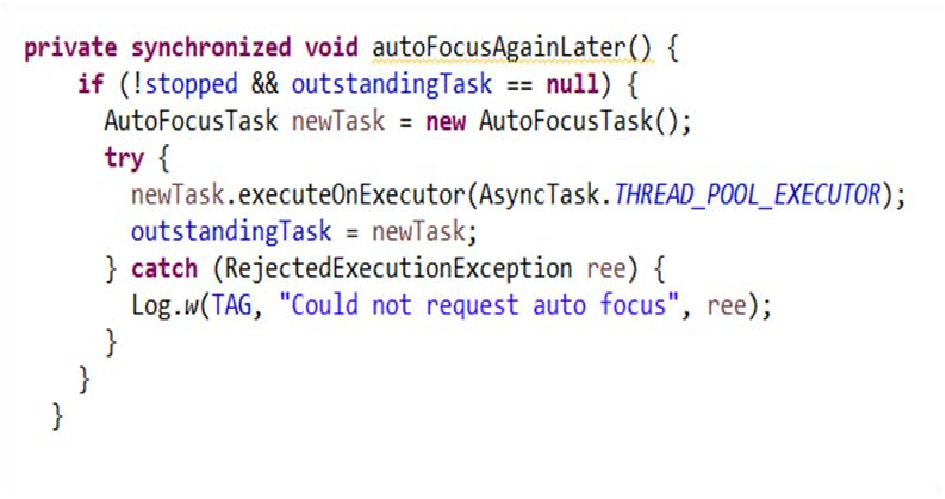
\includegraphics[width=\linewidth]{img/function.pdf}
% \caption{\label{figure:functionExample2}function example}
%\end{figure}

%\begin{figure}[!htp]
% \centering
% 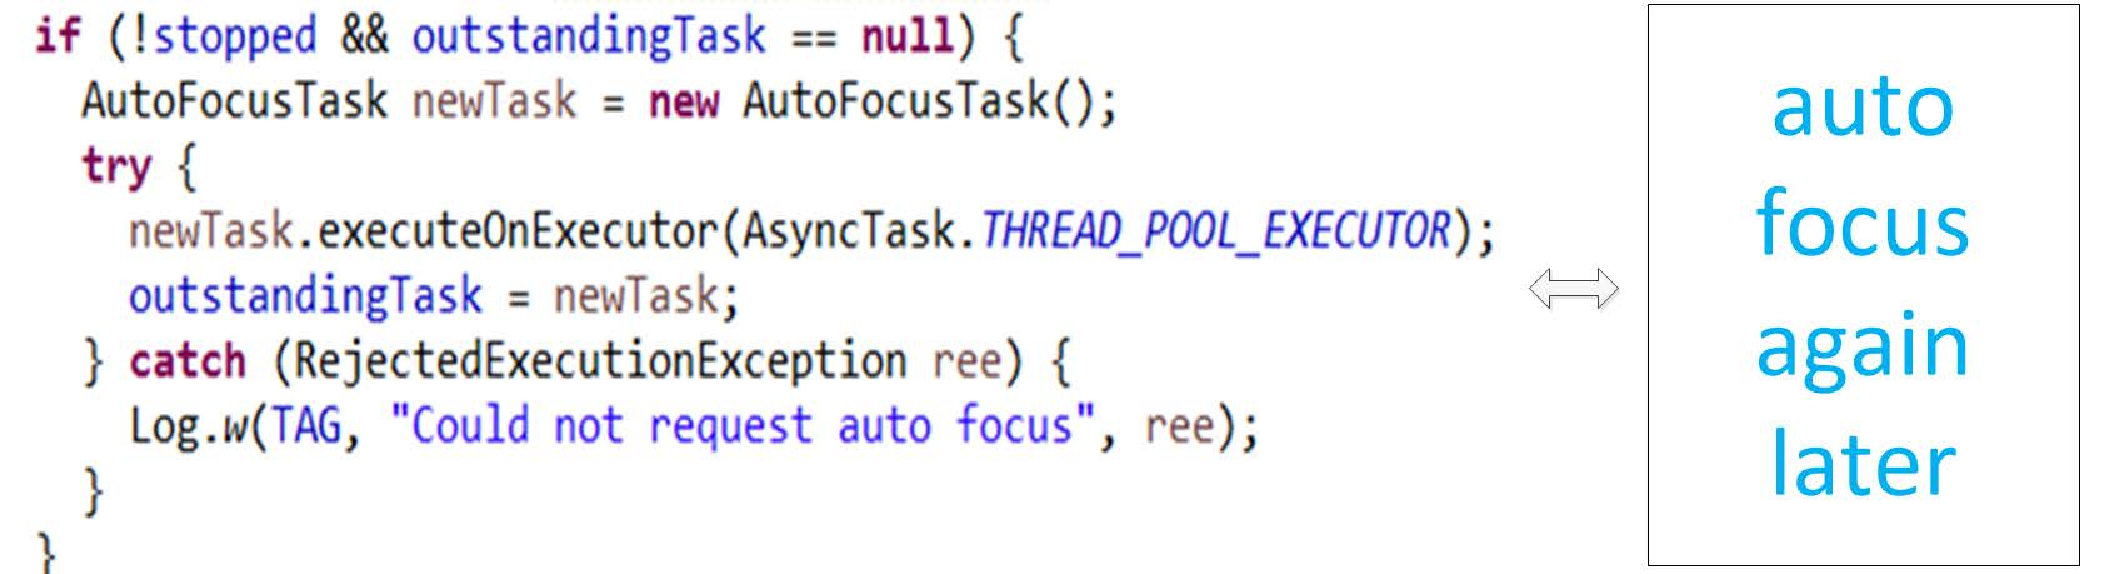
\includegraphics[width=\linewidth]{img/pair.pdf}
% \caption{\label{figure:pairExample} code and tag pair}
%\end{figure}

For every repository, we choose 100 functions and put their $(T,C)$ pairs
into the evaluation set. After that, we introduce the tags of another 49
functions $T$, as the negative noise, into every function's candidate set
of tags.
%And because we split all functions' name into individual words, every function may have almost 100 candidate tags.
Our task is to return the correct tags from all candidate tags.

\subsection{Baselines}
To show the effectiveness of our model, we compare against two baseline
approaches. These two baselines are both based on bag of word model
from the source code and don't utilize any structural information
such as parse tree and so on. Here a word refers to a token (which may or
may not be English) from the source code.

\subsubsection{TF-IDF}
We first extract all the identifiers and construct the bag of words
for every function without any modifications to the words.
% and add them into the vocabulary of repository.
%For every function, it has own word list, and if one identifier appears in function $n$ times, there will be also $n$ same identifiers in the word list.
Treating every function as a document, we compute TF-IDF score of each
word against every function and rank all words for every function by this
TF-IDF score.
%So we can get a vector to represent function and the value of this vector is the TF-IDF value of all words to this function. Meanwhile, we can get a similar vector for every tag. Finally, we calculate the cosine distance between functions and tags. We can rank all candidate tags according to cosine distance for every function.

\begin{figure}[ht]
 \centering
 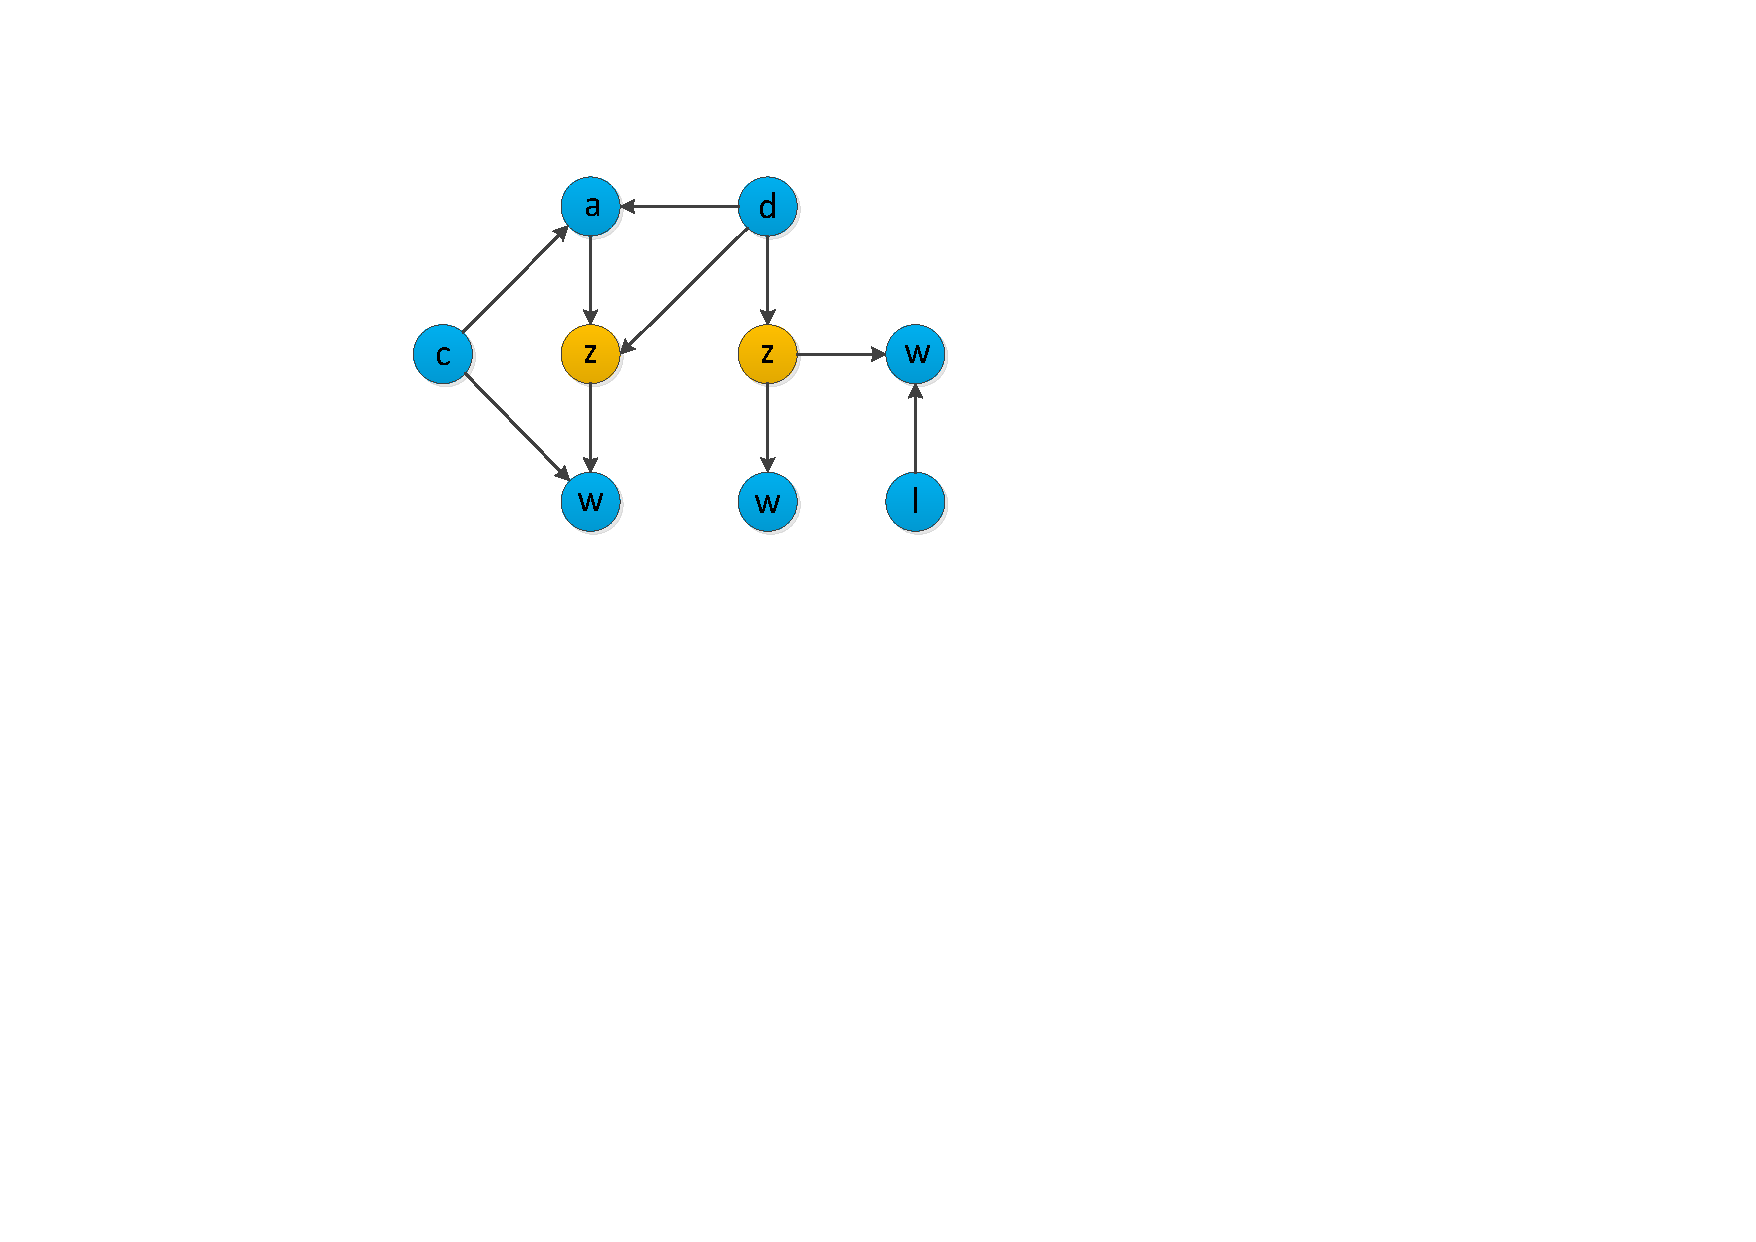
\includegraphics[width=0.5\linewidth]{img/probabilisticModel.pdf}
 \caption{\label{figure:probModel}Probabilistic Graphical Model for Code Repo}
\end{figure}

\subsubsection{Topic Model}\label{sec:topicModel}
%In this baseline, %we choose the same method to extract the vocabulary and the word list of every function as above. Then
We construct a probabilistic graphical model for each code repository.
As shown in Fig \ref{figure:probModel}, $d$ is a source code function,
$z$ is the topic of $d$, $w$ is the word that may appear in $d$,
$l$ is the programming language and $c$ means the comment of $d$.
Then we can generate a function following two steps:
\begin{itemize}
    \item generate one subject $z$ following the multinomial distribution $multi(z|d)$ with the fixed function $d$.
    \item generate one word that might appear in function $d$, following
the multinomial distribution $multi(w|z)$ conditioned on $z$,
which was generated in the previous step.
\end{itemize}
We thus generate one word for function $d$ after the two steps.
We can then get all words of $d$ after iterating many times.
%And if we iterate these two steps many times, we can get the whole function $d$.
Next, we use the EM algorithm to train our probabilistic model and
gain the distribution of $P(z|d)$ and $P(w|z)$.
Finally we get $P(w|d)=P(w|z)*P(z|d)$ and rank all words for every method
based on $P(w|d)$.
%The equation of calculating probabilistic is:
%\begin{equation}
%    {
%    \begin{split}
%        P(Data|\phi)=\prod_{m}\prod_{i}\Big(\eta \sum_{k}P(w_{i}|z_{k})P(z_{k}|d_{m})+\\
%        (1-\eta)P(w_{i}|s)\Big)^{l(w_{i}^{(x)},d_{m})} \\
%        \prod_{j}\Big(\sum_{k}P(w_{j}|z_{k})P(z_{k}|d_{m})\Big)^{l(w_{j}^{(y)},d_{m})}
%    \end{split}
%    }
%\end{equation}
%where $Data$ is the data of function and $\phi$ is all situations that functions may meet. $l$ is the function that count the time of word $w_{i}$ appears.
%
%Following is the equation of our EM algorithm:
%\begin{itemize}
%\item E step:
%\begin{equation}
%{
%    P(z_{k}\ |\ w_{i},d_{m})  = \frac{P(w_{i}\ |\ z_{k})P(z_{k}\ |\ d_{m})}{\sum_{k}P(w_{i}\ |\ z_{k})P(z_{k}\ |\ d_{m})}
%}
%\end{equation}
%\item M step:
%\begin{equation}
%{
%    l(w_{i},d_{m}) = \eta l(w_{i}^{(x)},d_{m})+l(w_{i}^{(y)},d_{m})
%}
%\end{equation}
% \ To compute $P(w_{i}|z_{k})$
%
%\begin{equation}
%{
%\begin{split}
%    P(w_{i}|z_{k})  =
%  \frac{ \sum_{m}\alpha l(w_{i},d_{m})P(z_{k}|w_{i},d_{m})}
%  {\sum_{i} \sum_{m} \alpha l(w_{i},d_{m})P(z_{k}|w_{i},d_{m})}\\
%  \frac{ +(1-\alpha)l(w_{i},d_{m})\sum_{m^{'}}\beta_{m,m^{'}}P(z_{k}|w_{i},d_{m^{'}})}{ +(1-\alpha)l(w_{i},d_{m})\sum_{m^{'}}\beta_{m,m^{'}}P(z_{k}|w_{i},d_{m^{'}}) }
%\end{split}
%}
%\end{equation}
%
% \ To compute $P(z_{k}|d_{m})$
%
%{
%\begin{align}
%\begin{split}
%    P(z_{k}|d_{m})  =
%  \frac{ \sum_{i}\alpha l(w_{i},d_{m})P(z_{k}|w_{i},d_{m})}
%  {\sum_{k} \sum_{i} \alpha l(w_{i},d_{m})P(z_{k}|w_{i},d_{m})}\\
%  \frac{ +(1-\alpha)\sum_{n}l(w_{i},d_{n})\beta_{n,m}P(z_{k}|w_{i},d_{n})}{ +(1-\alpha)\sum_{n}l(w_{i},d_{n})\beta_{n,m}P(z_{k}|w_{i},d_{n}) }
%\end{split}
%\end{align}
%}
%
%\end{itemize}

\subsection{Results}\label{sec:result}

\subsubsection{Accuracy}
We calculate the accuracy of each of the four competing models
as :
\begin{equation}
{
  accuracy  = \frac{\sum_{i=1}^{k}1(pos_{i} \leq n)}{k}
}
\end{equation}
where $pos_{i}$ is the position of $tag_{i}$ in ranked tag list,
$n$ is the number of tags that we want to choose and
$k$ is the number of tags in the ground truth.
The function $1(pos_{i} \leq n)$ means if $pos_{i} \leq n$
is true then return 1, else return 0.

In this part, we use every single word as our tag to evaluate our model
and these single words are all split from methods' name. We do this
so that we can compare our model with TF-IDF and topic model, both of which are
based on bag of words. Every method has almost 100 candidate tags
because most method names can be split into two or three single words.

For example, we have in total 10 tags in the list and 2 tags $tag_{1}$
and $tag_{2}$ in groundtruth. The position of $tag_{1}$ and $tag_{2}$
are second and seventh position respectively.
If we only choose 5 tags from the tag list,
the accuracy will be 0.5 ($\frac{1+0}{2}=0.5$).
%Fig \ref{figure:accuracyOfFour} shows the result of four model when we choose 5 and 10 tags from candidate tags.
 %We can see that there are four histograms that represent the accuracy of four models respectively.
%four different color lines for different number of tags. The red line is the accuracy of our model, green one is the result of Miltiadis's model, the blue line shows the accuracy of our topic model baseline and finally the black line is the accuracy of TF-IDF model. The different color rectangle measures the approvement between this model and the previous one. For example, the red rectangle measures the increase between our model and Miltiadis's model. The larger the area, the greater the increase.
%From Fig \ref{figure:accuracyOfFour} we can know our model is the best one and the improvement between Allamanis et al's model and topic model is the largest one.
Fig \ref{figure:accuracyOfDiffTags} shows the accuracy of four models
when we range $k$ from 1 to 50. The results of our model and Allamanis' model
are both obtained after the
sixth iteration of training. Clearly, our new model is better than the other three models in most repositories.
In repository {\em mockito}, our model is almost the same as
Allamanis' at sixth iteration, because this repo tends to use very long
identifiers such as ``shouldSayTooLittleInvocationsInAtLeastMode'',
which carry a lot of unnecessary semantic information (e.g., ``should'' and
``say'') and thus confuse the model.
%This suggests that our model, which contains more information,
%requires longer time to converge.
%We can see our model is always better than Allamanis et al's model. And when we choose 50 tags, accuracy is almost 0.9, so we can say that most of our tags are at the first half position(every function has 100 candidate tags).
%\begin{figure*}[!htp]
% \centering
%  \begin{minipage}{0.18\linewidth}
% 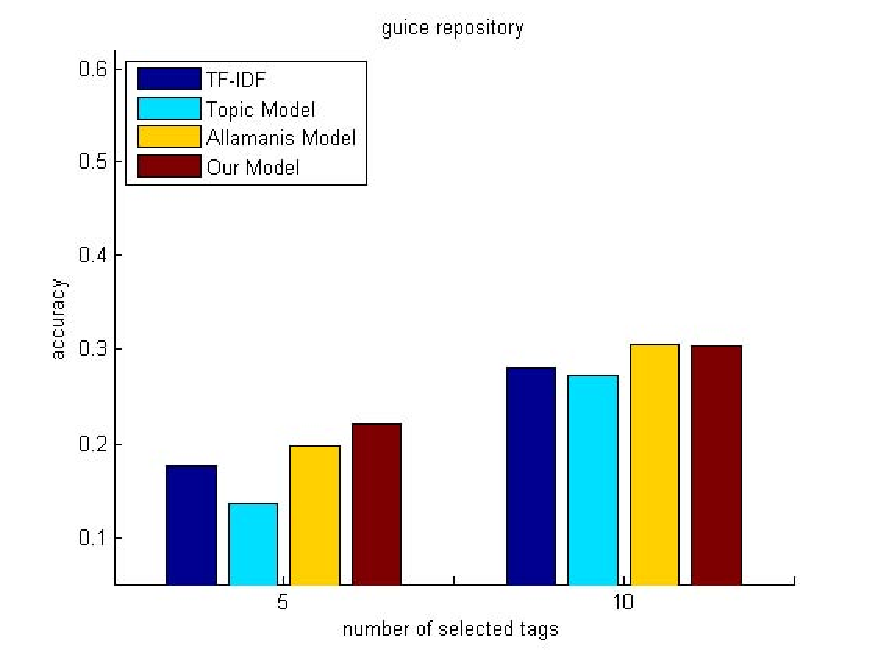
\includegraphics[width=\linewidth]{img/guiceBar.pdf}
% \end{minipage}
% \hfill
% \begin{minipage}{0.18\linewidth}
% 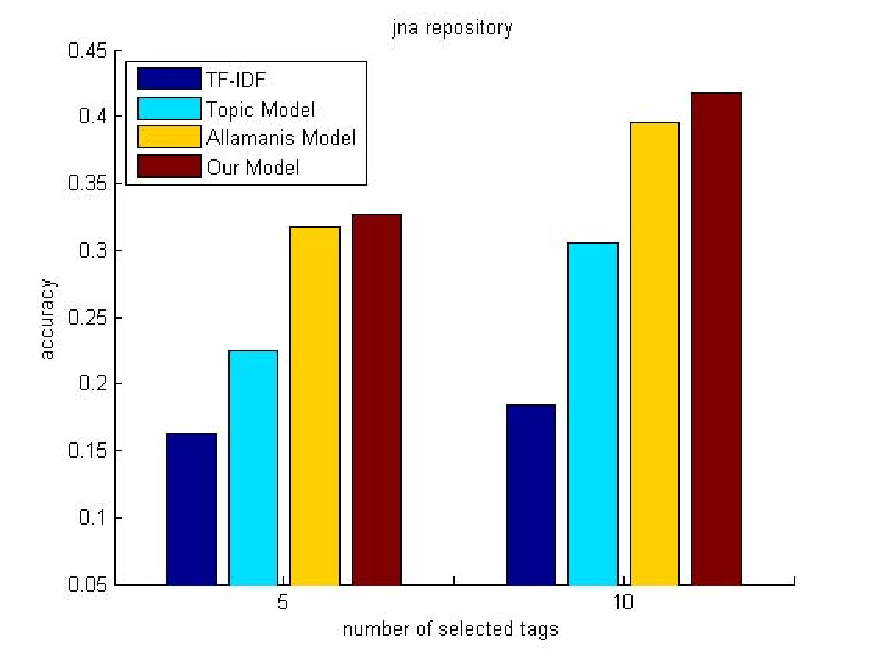
\includegraphics[width=\linewidth]{img/jnaBar.pdf}
% \end{minipage}
% \hfill
% \begin{minipage}{0.18\linewidth}
% 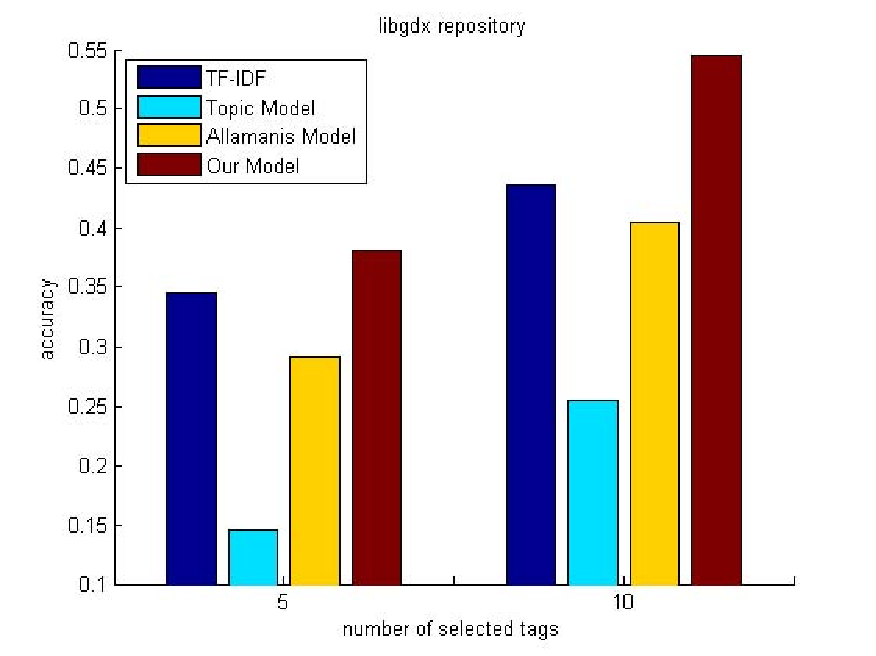
\includegraphics[width=\linewidth]{img/libgdxBar.pdf}
% \end{minipage}
% \hfill
% \begin{minipage}{0.18\linewidth}
% 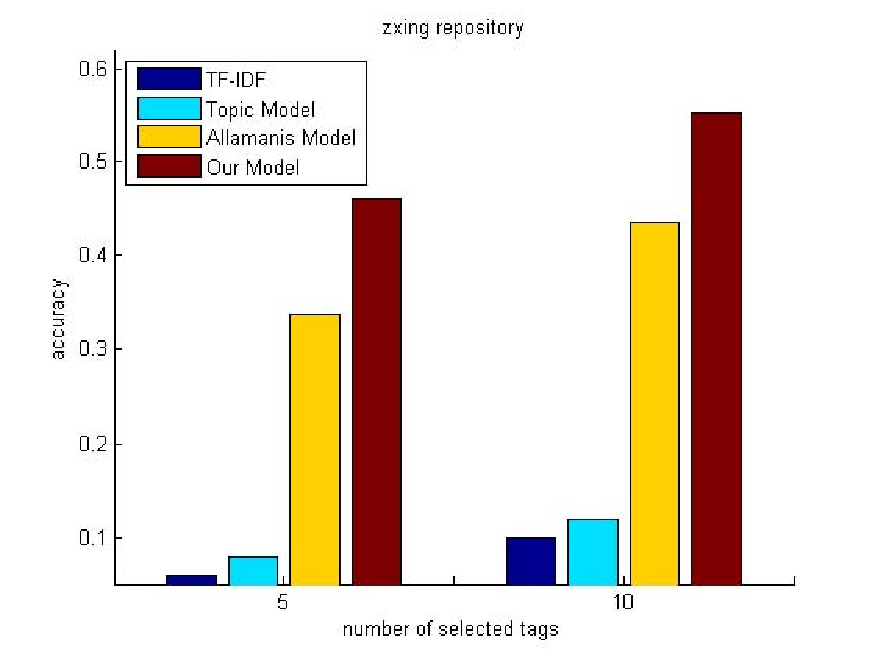
\includegraphics[width=\linewidth]{img/zxingBar.pdf}
% \end{minipage}
% \hfill
% \begin{minipage}{0.18\linewidth}
% 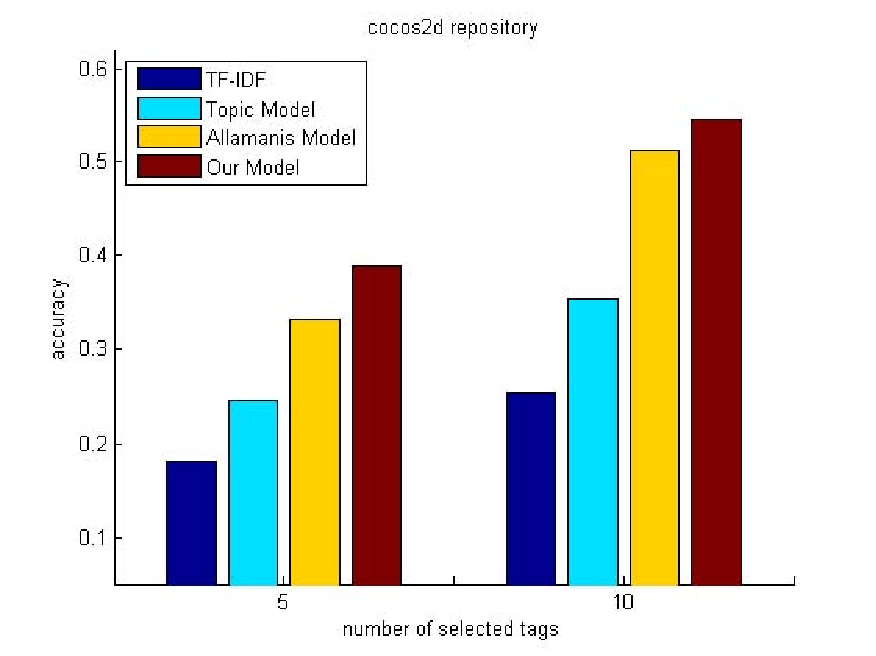
\includegraphics[width=\linewidth]{img/cocos2dBar.pdf}
% \end{minipage}
%
% \vfill
%
% \begin{minipage}{0.18\linewidth}
% 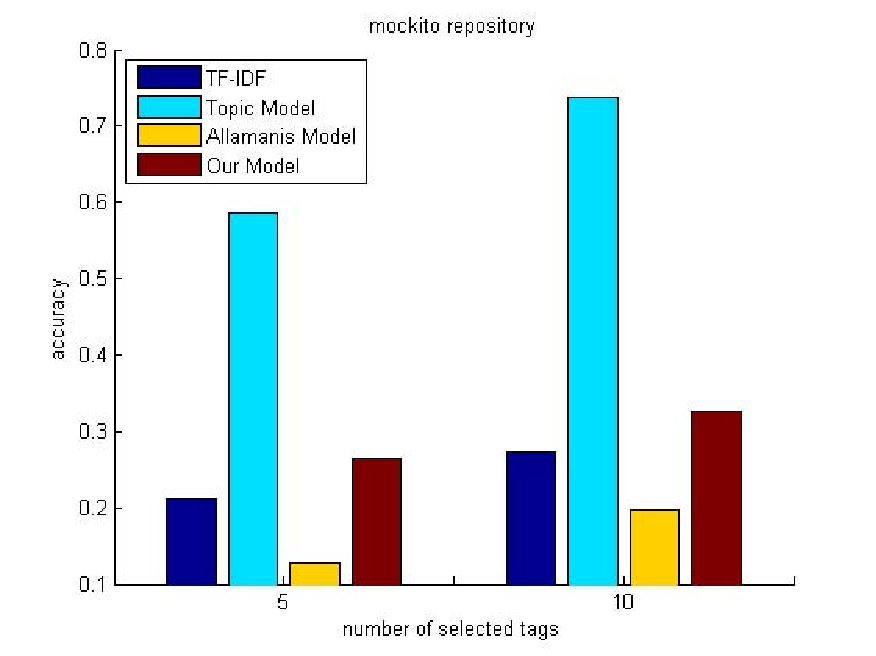
\includegraphics[width=\linewidth]{img/mockitoBar.pdf}
% \end{minipage}
% \hfill
% \begin{minipage}{0.18\linewidth}
% 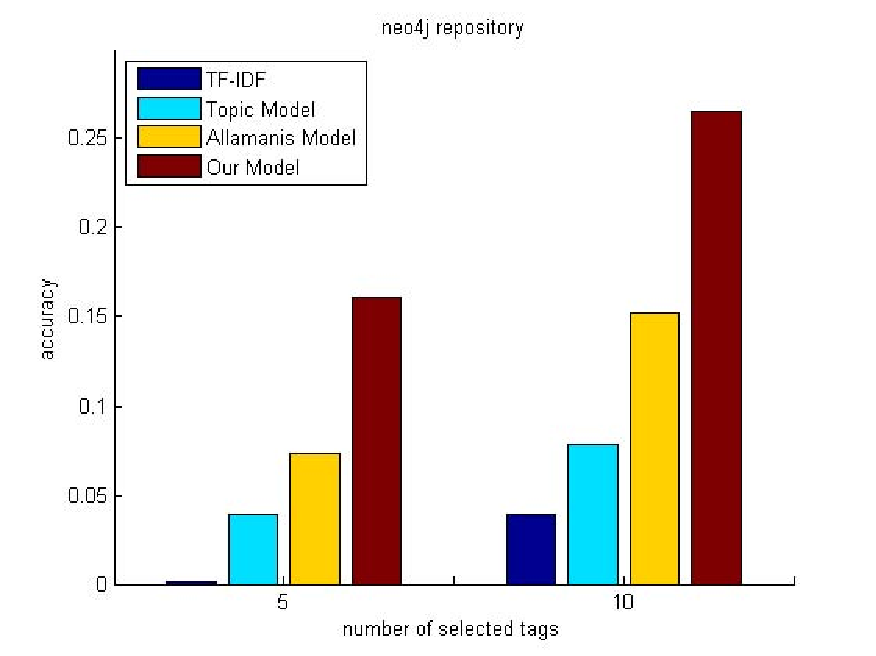
\includegraphics[width=\linewidth]{img/neo4jBar.pdf}
% \end{minipage}
% \hfill
% \begin{minipage}{0.18\linewidth}
% 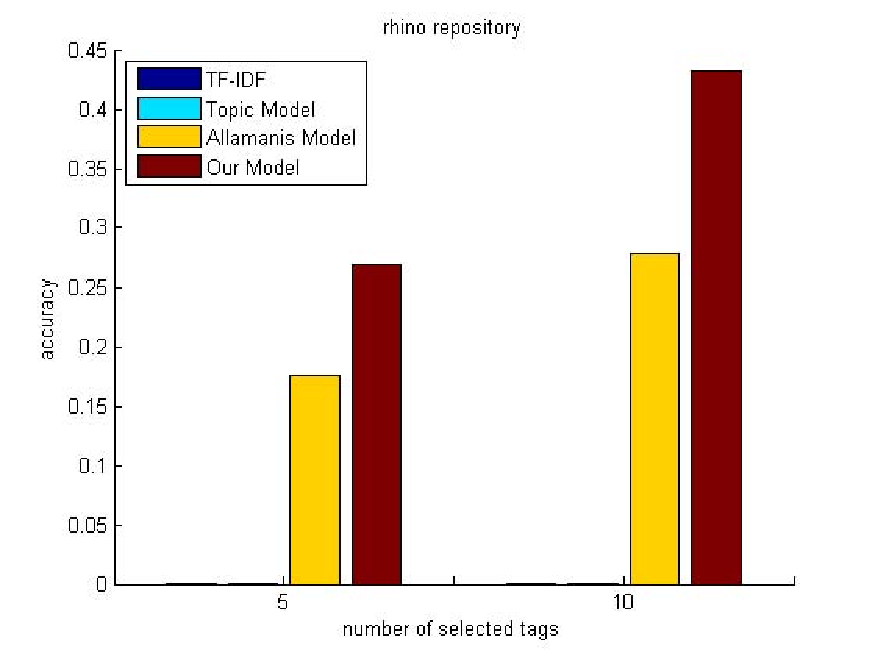
\includegraphics[width=\linewidth]{img/rhinoBar.pdf}
% \end{minipage}
% \hfill
% \begin{minipage}{0.18\linewidth}
% 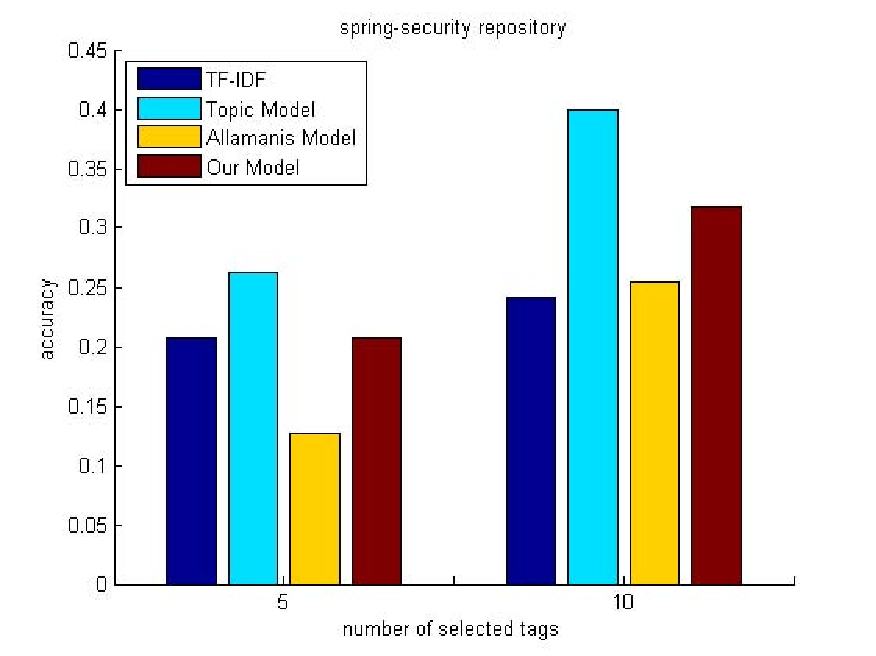
\includegraphics[width=\linewidth]{img/spring-securityBar.pdf}
% \end{minipage}
% \hfill
% \begin{minipage}{0.18\linewidth}
% 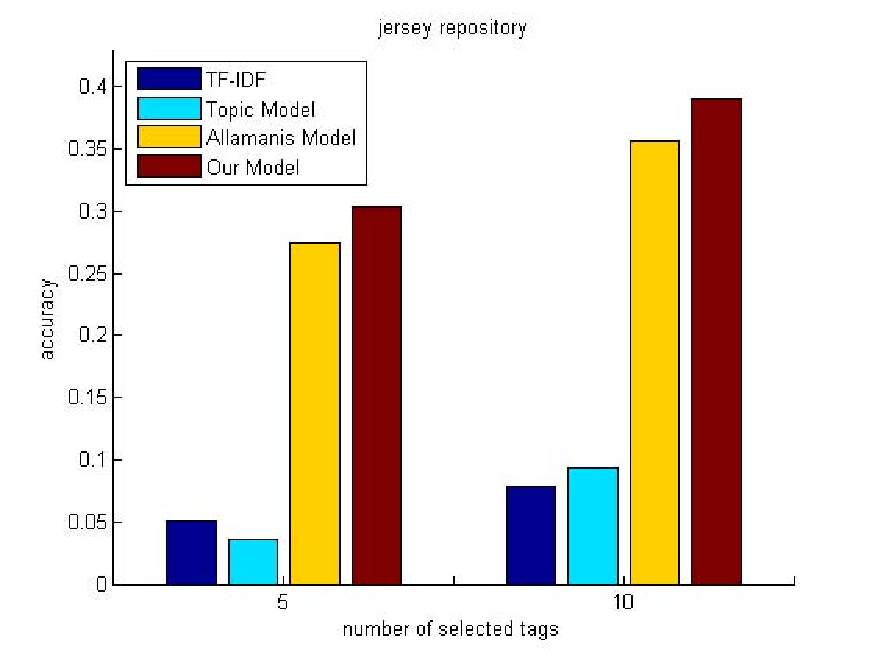
\includegraphics[width=\linewidth]{img/jerseyBar.pdf}
% \end{minipage}
% \caption{\label{figure:accuracyOfFour} accuracy of four model}
%\end{figure*}

\begin{figure}[!ht]
 \centering
 \begin{minipage}{0.40\linewidth}
 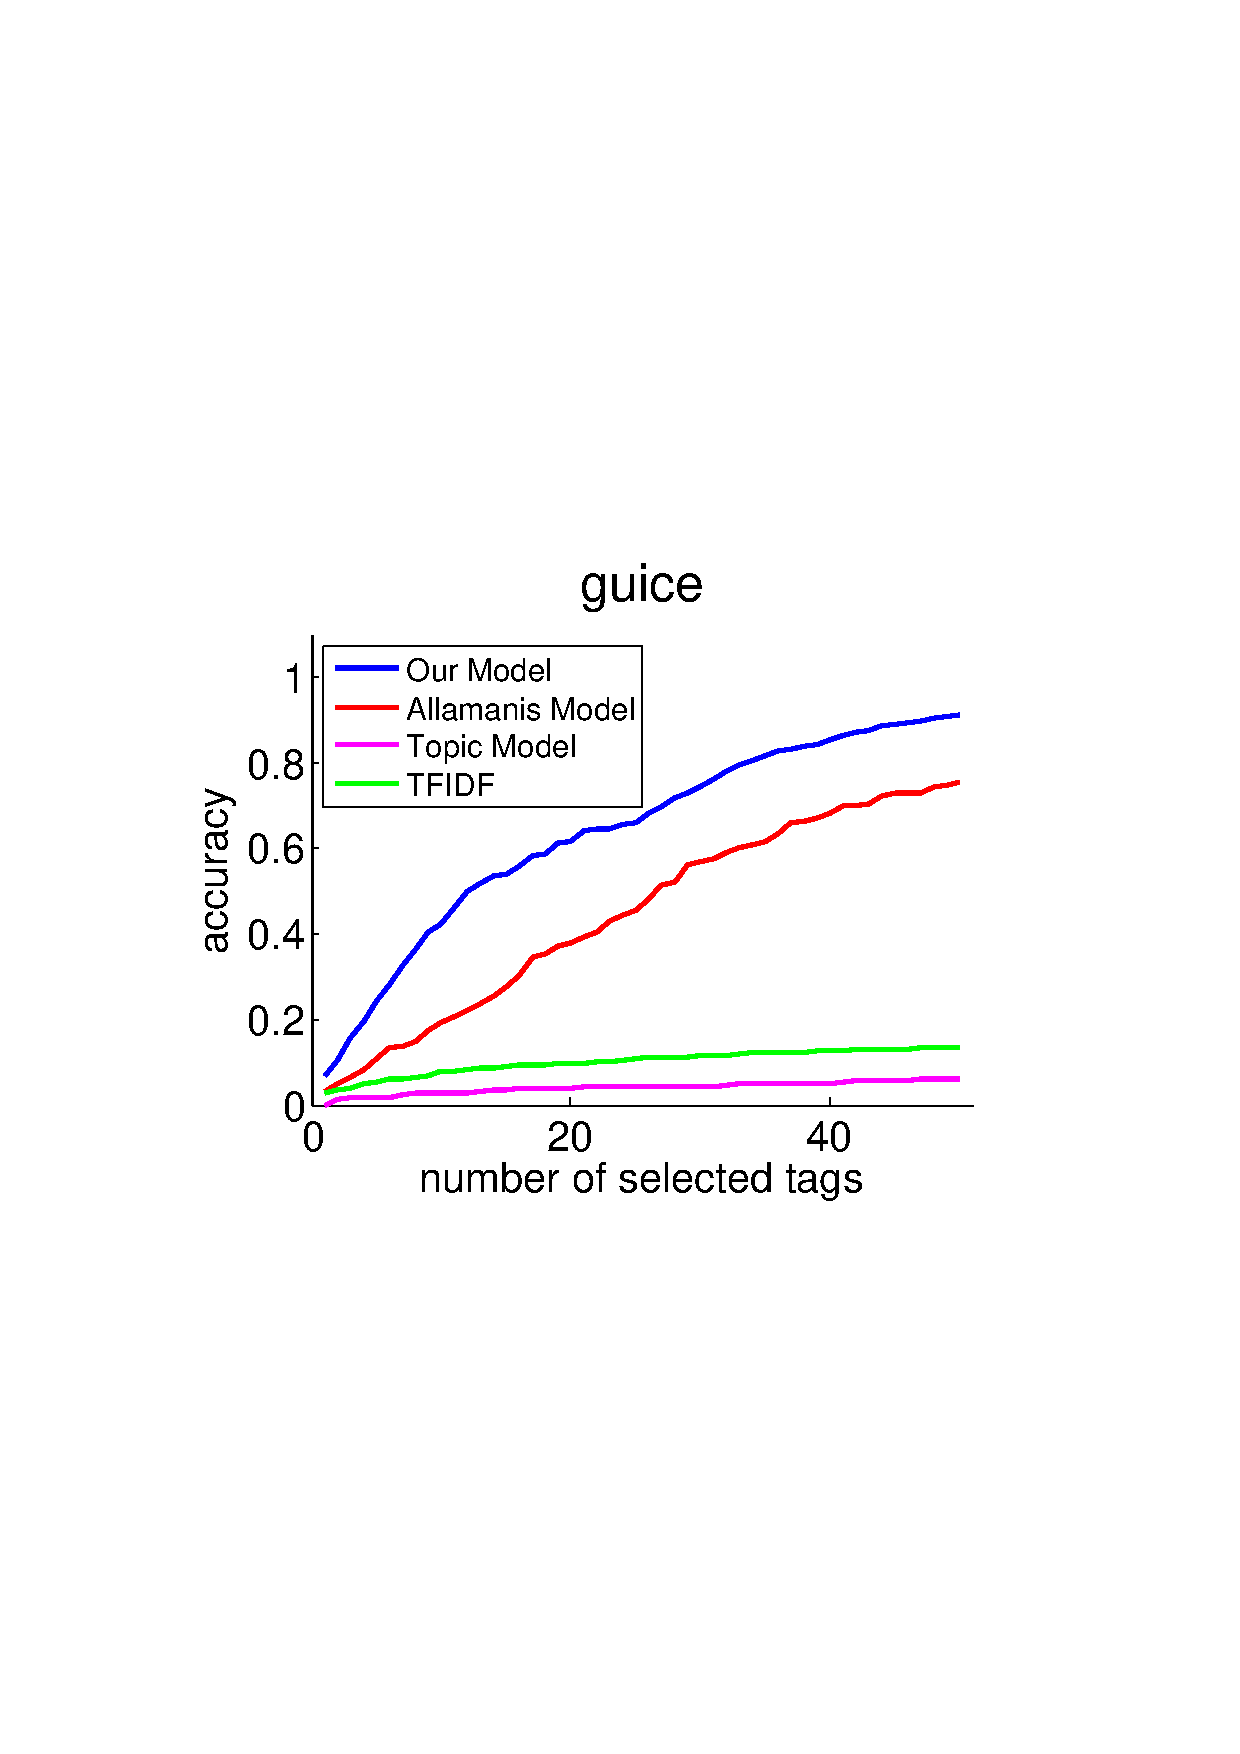
\includegraphics[width=\linewidth]{img/guiceLine.pdf}
 \end{minipage}
 \hfill
 \begin{minipage}{0.40\linewidth}
 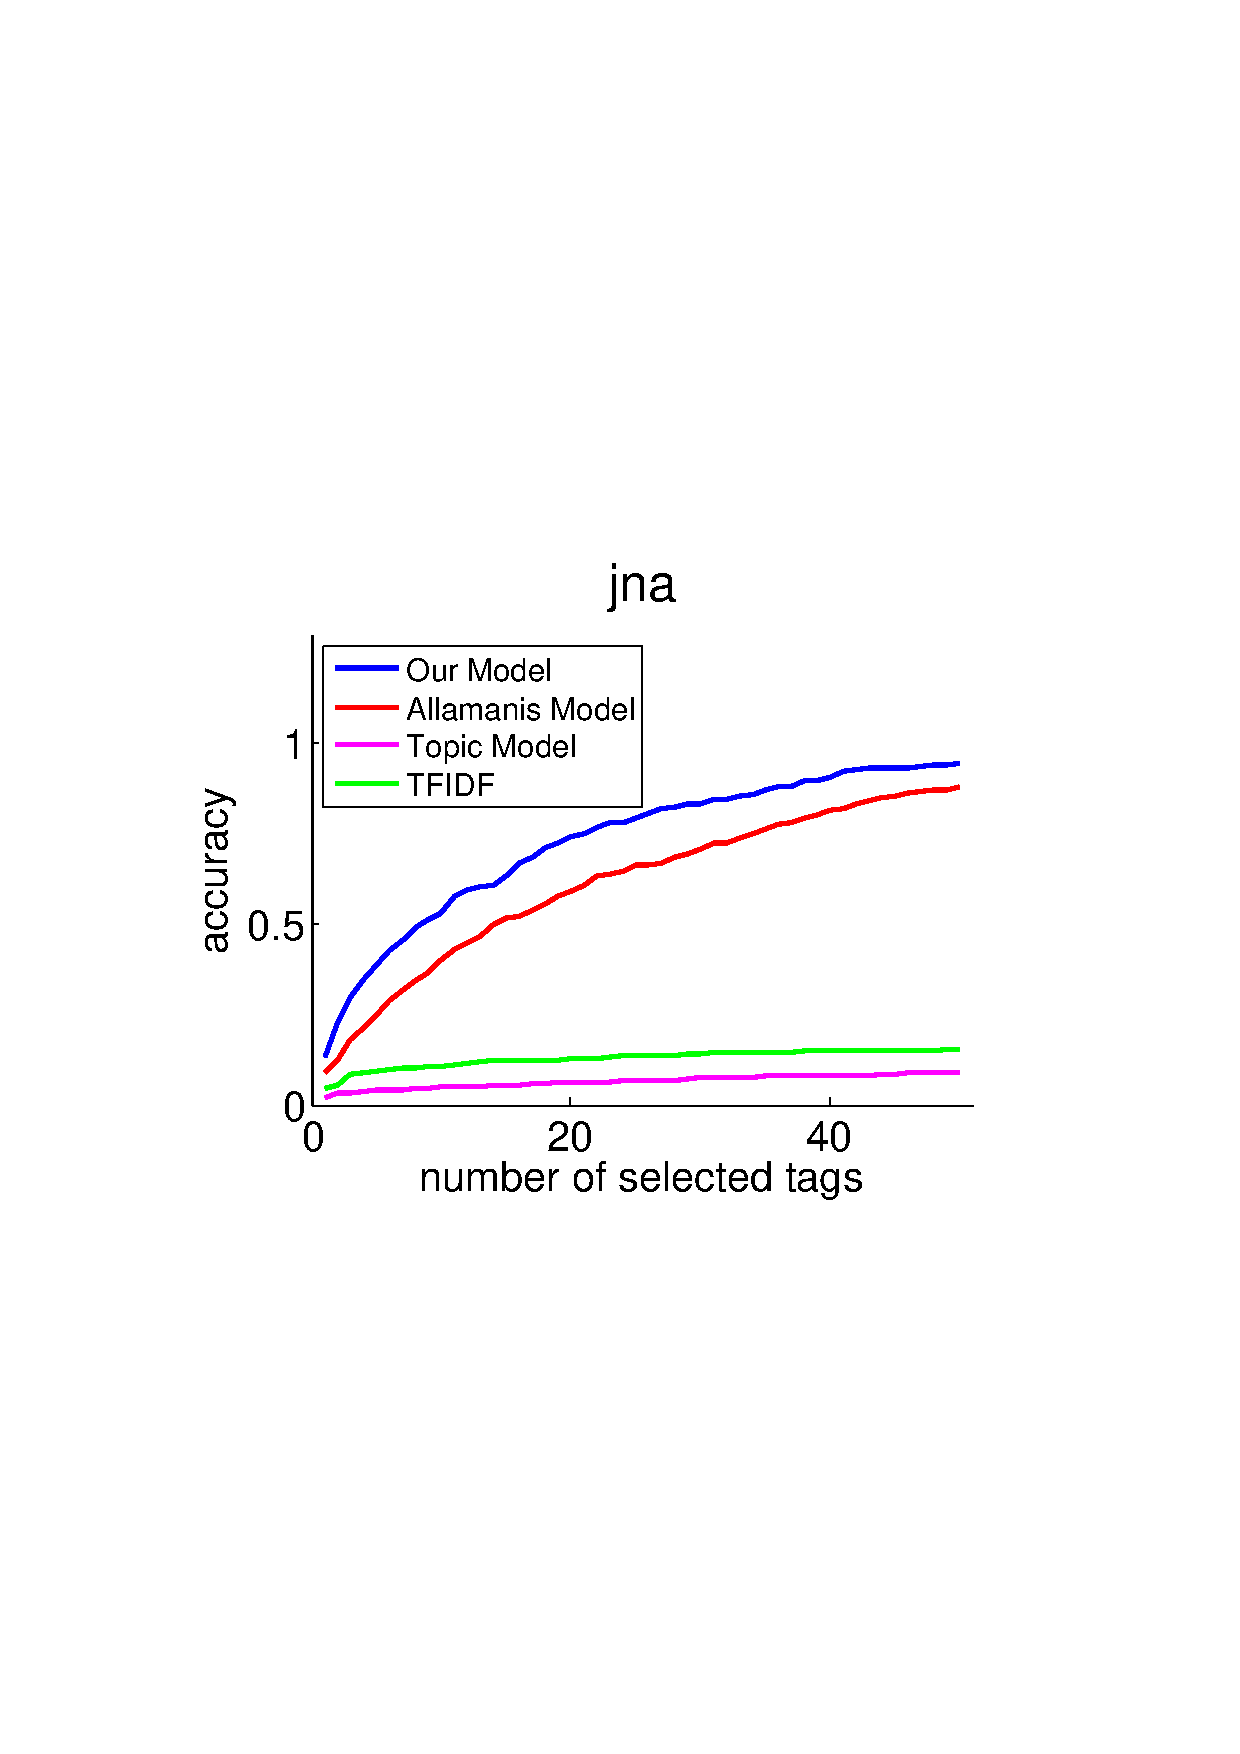
\includegraphics[width=\linewidth]{img/jnaLine.pdf}
 \end{minipage}
 \vfill
 \begin{minipage}{0.40\linewidth}
 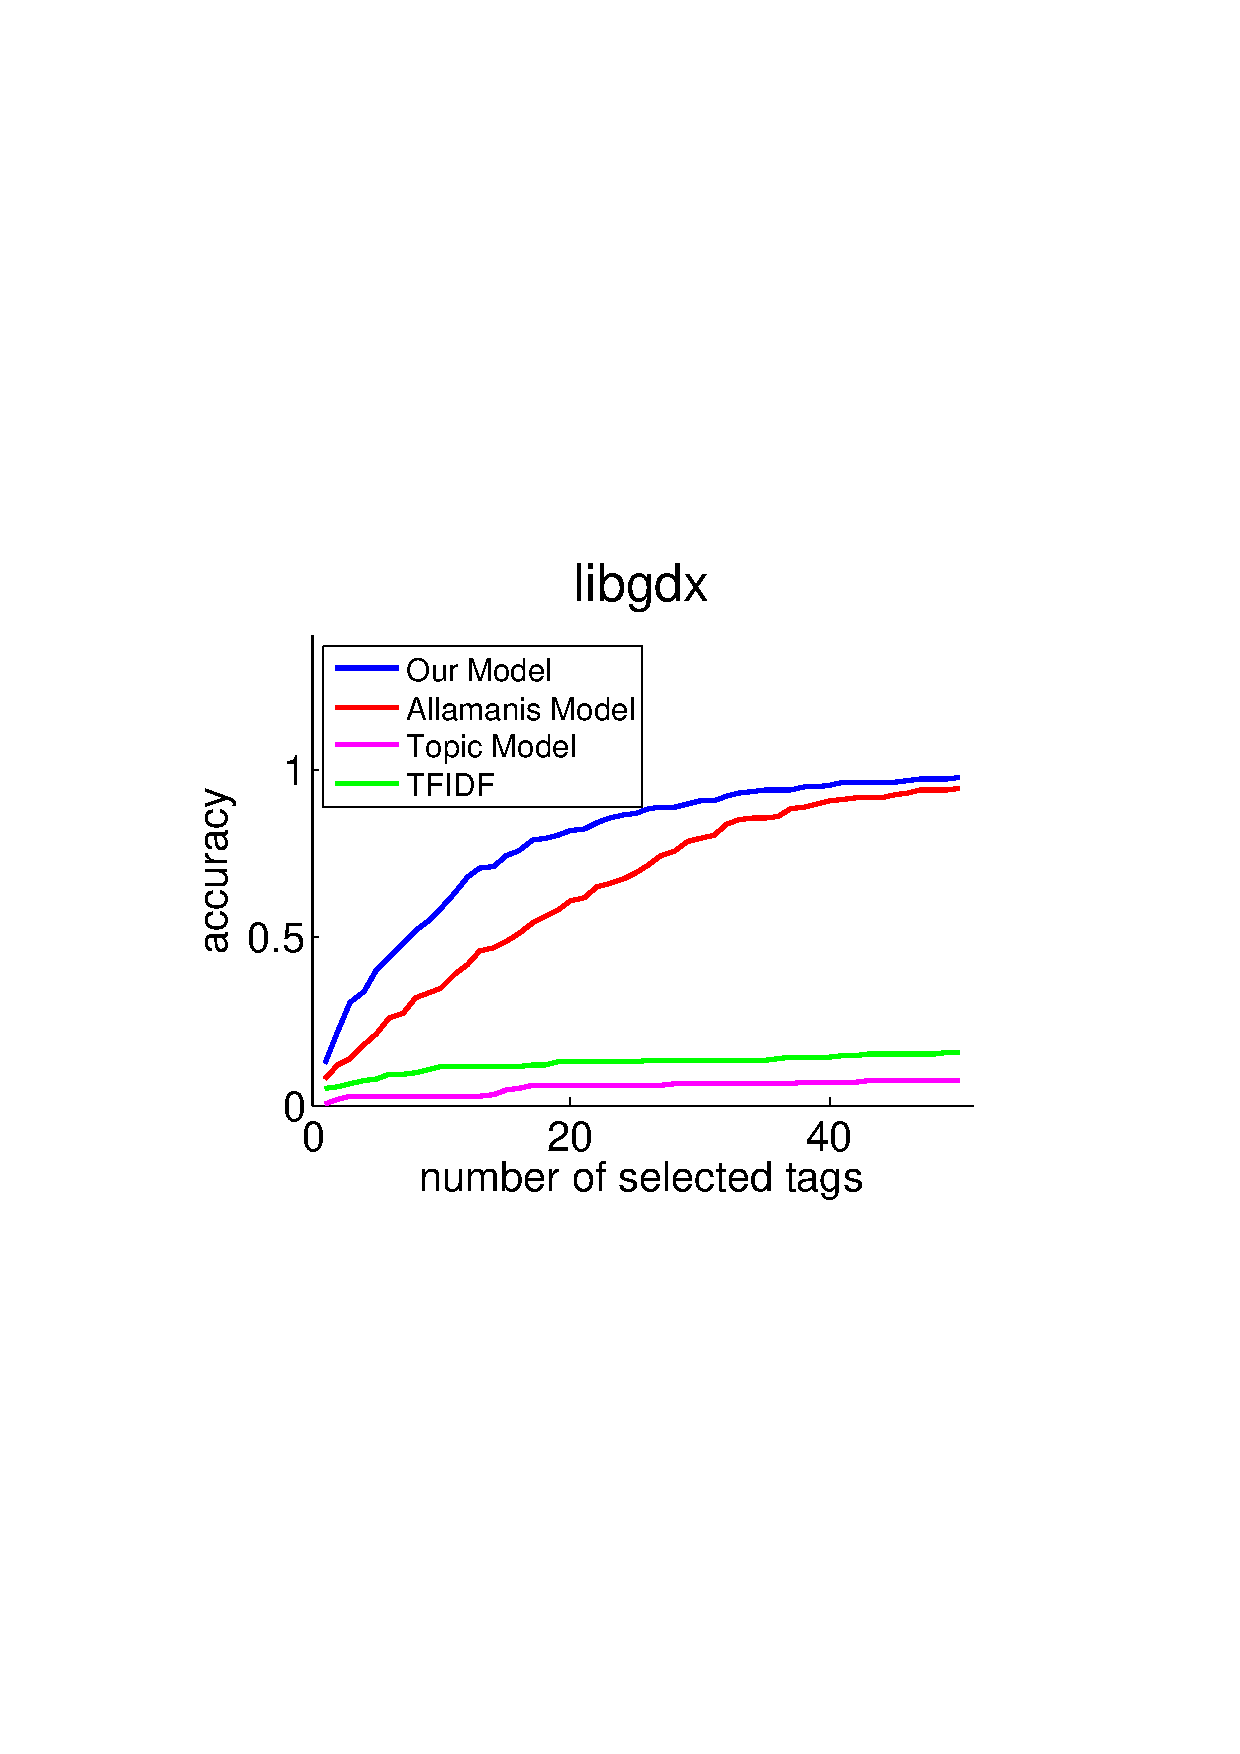
\includegraphics[width=\linewidth]{img/libgdxLine.pdf}
 \end{minipage}
 \hfill
 \begin{minipage}{0.40\linewidth}
 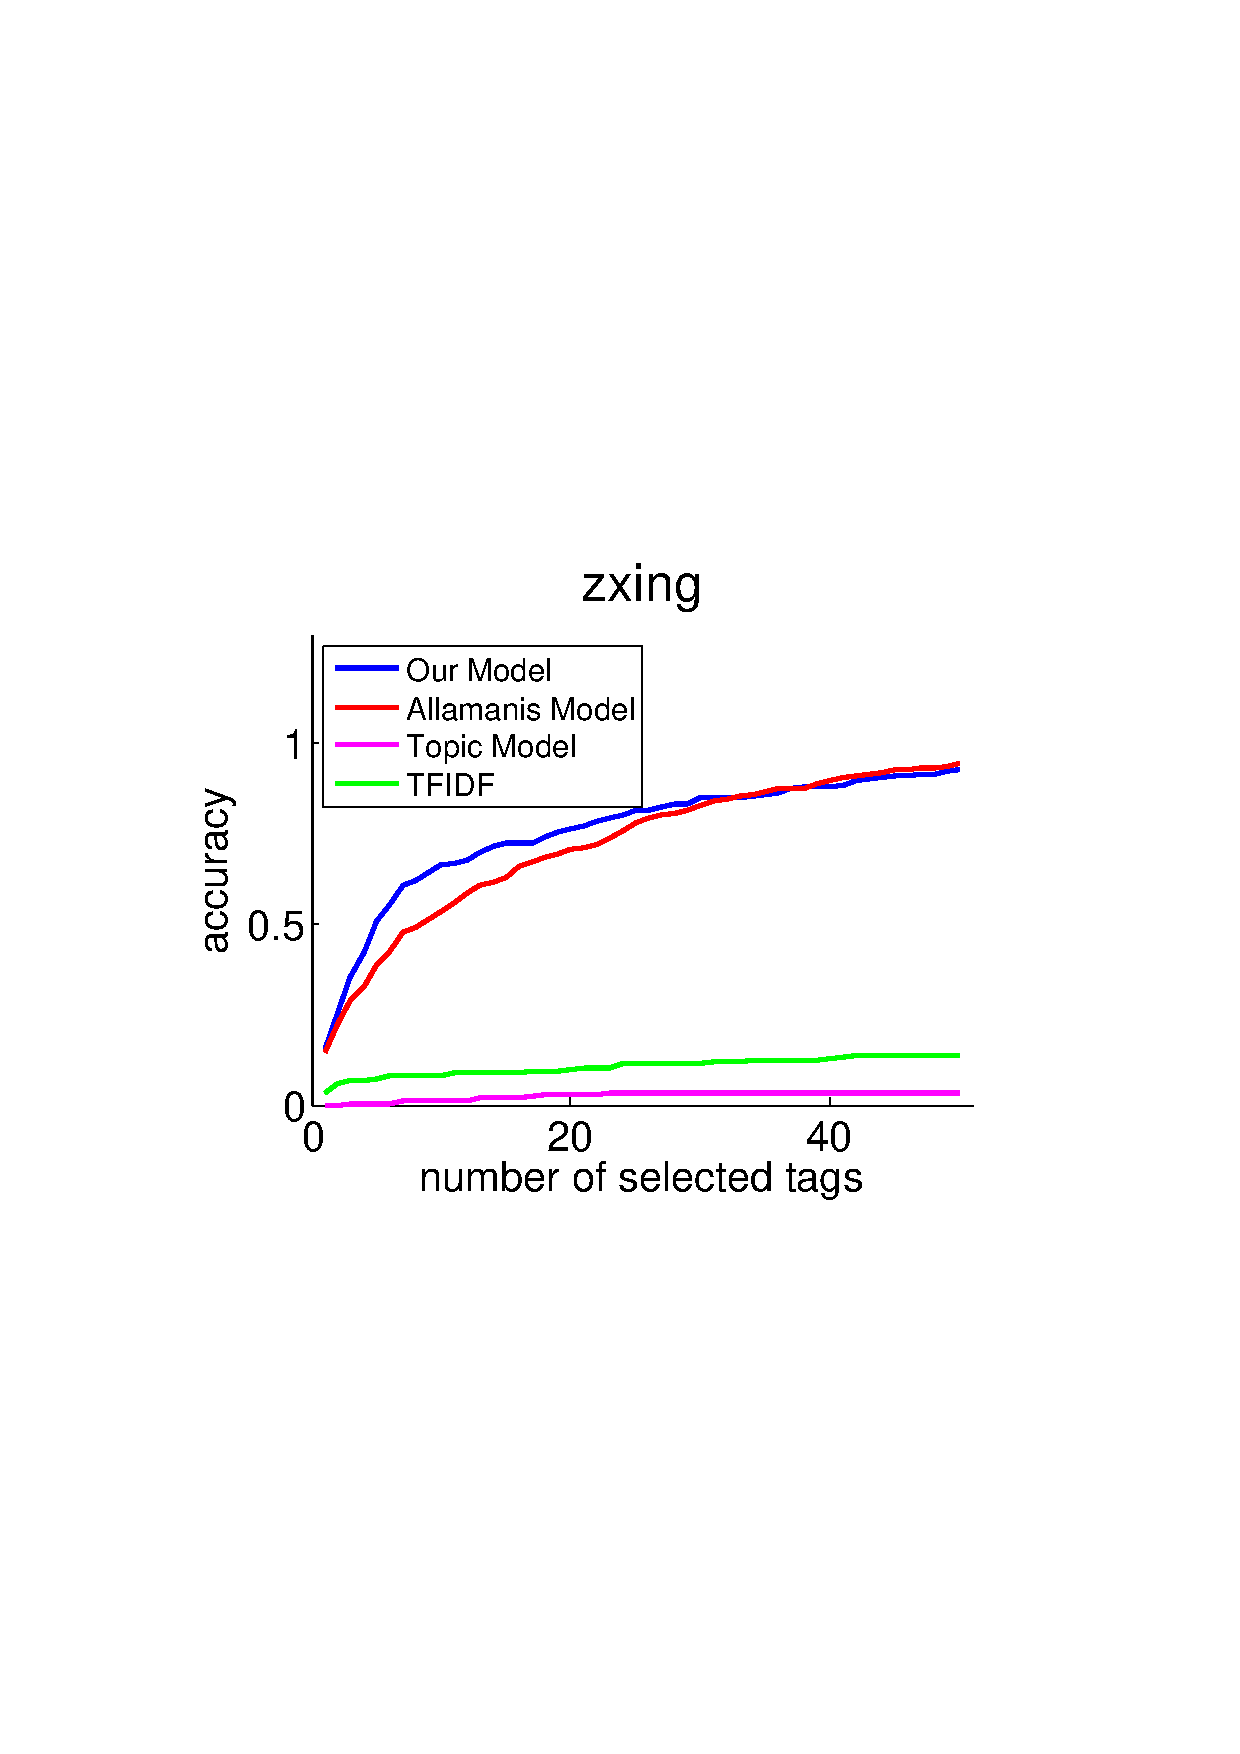
\includegraphics[width=\linewidth]{img/zxingLine.pdf}
 \end{minipage}
 \vfill
 \begin{minipage}{0.40\linewidth}
 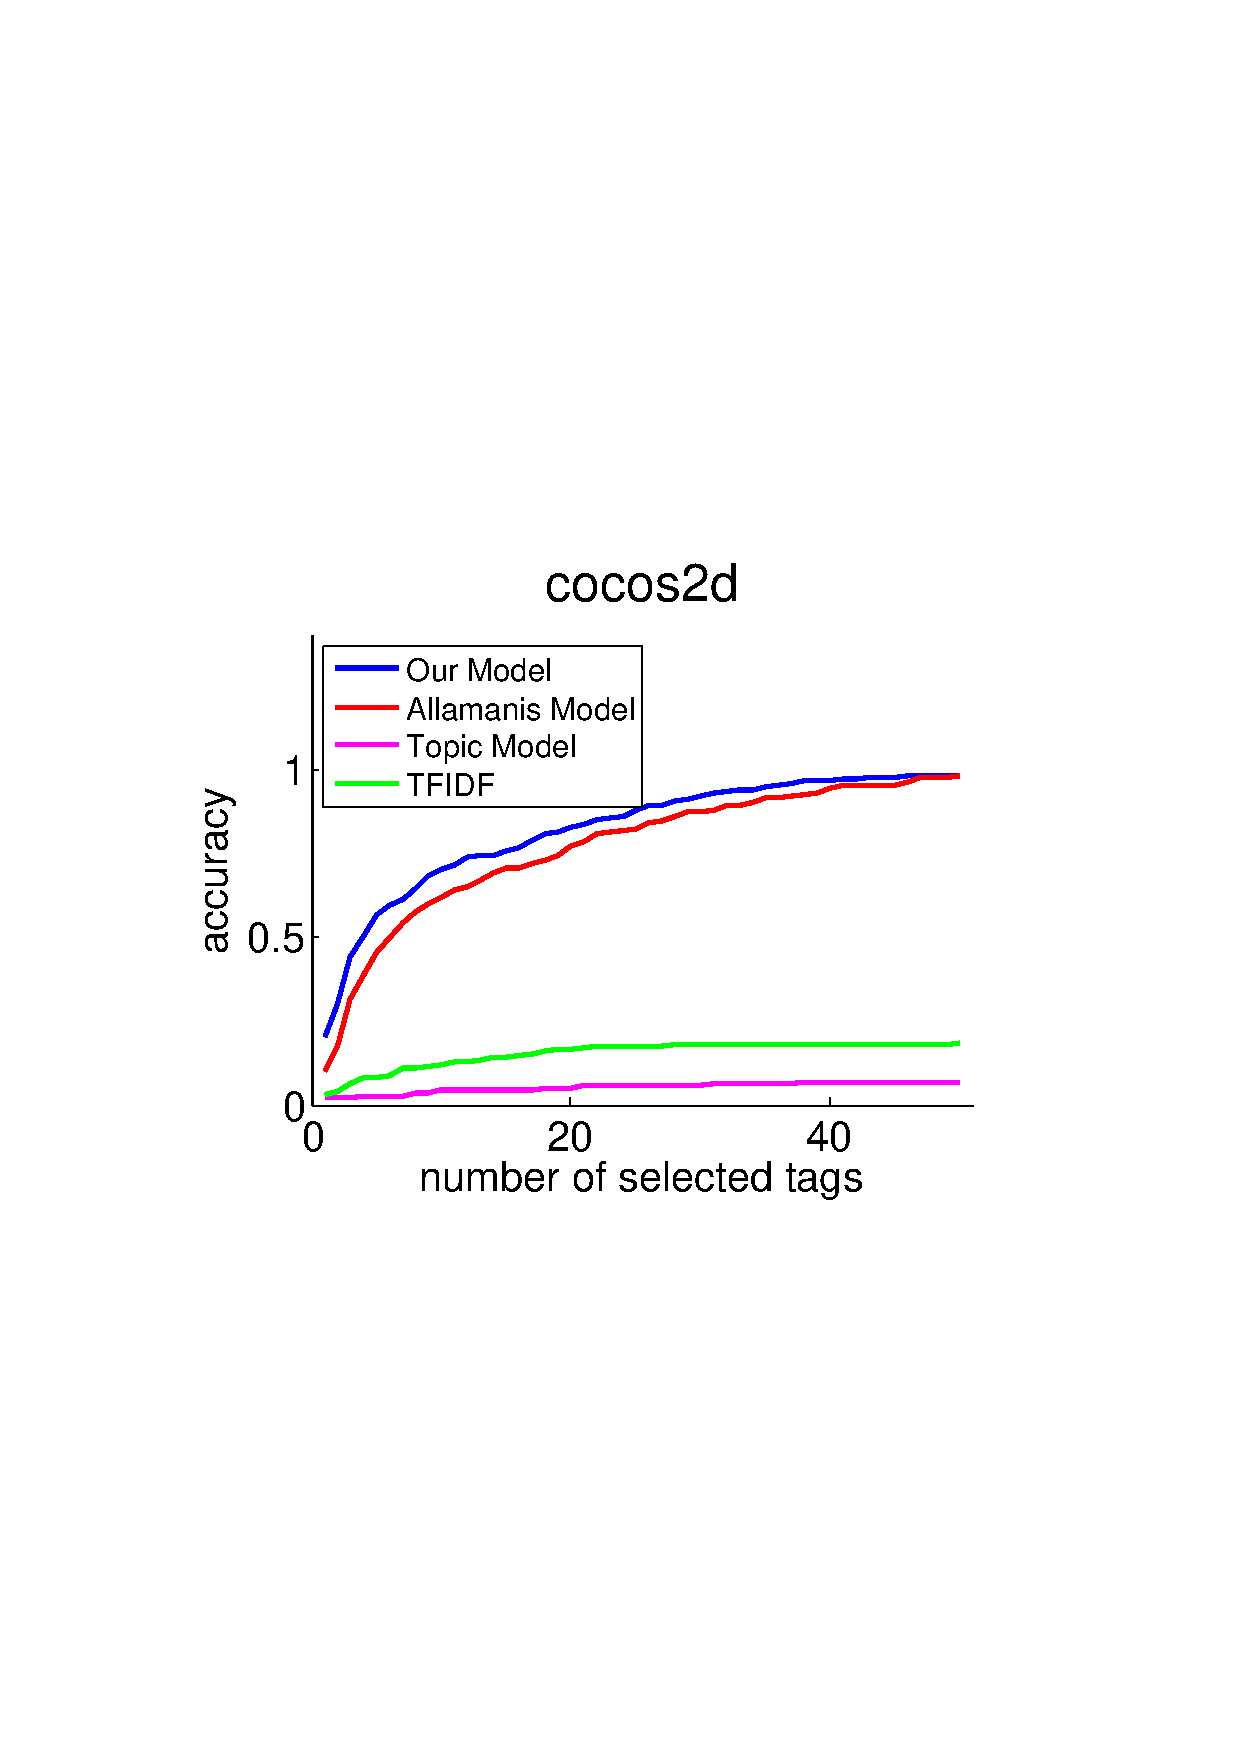
\includegraphics[width=\linewidth]{img/cocos2dLine.pdf}
 \end{minipage}
 \hfill
 \begin{minipage}{0.40\linewidth}
 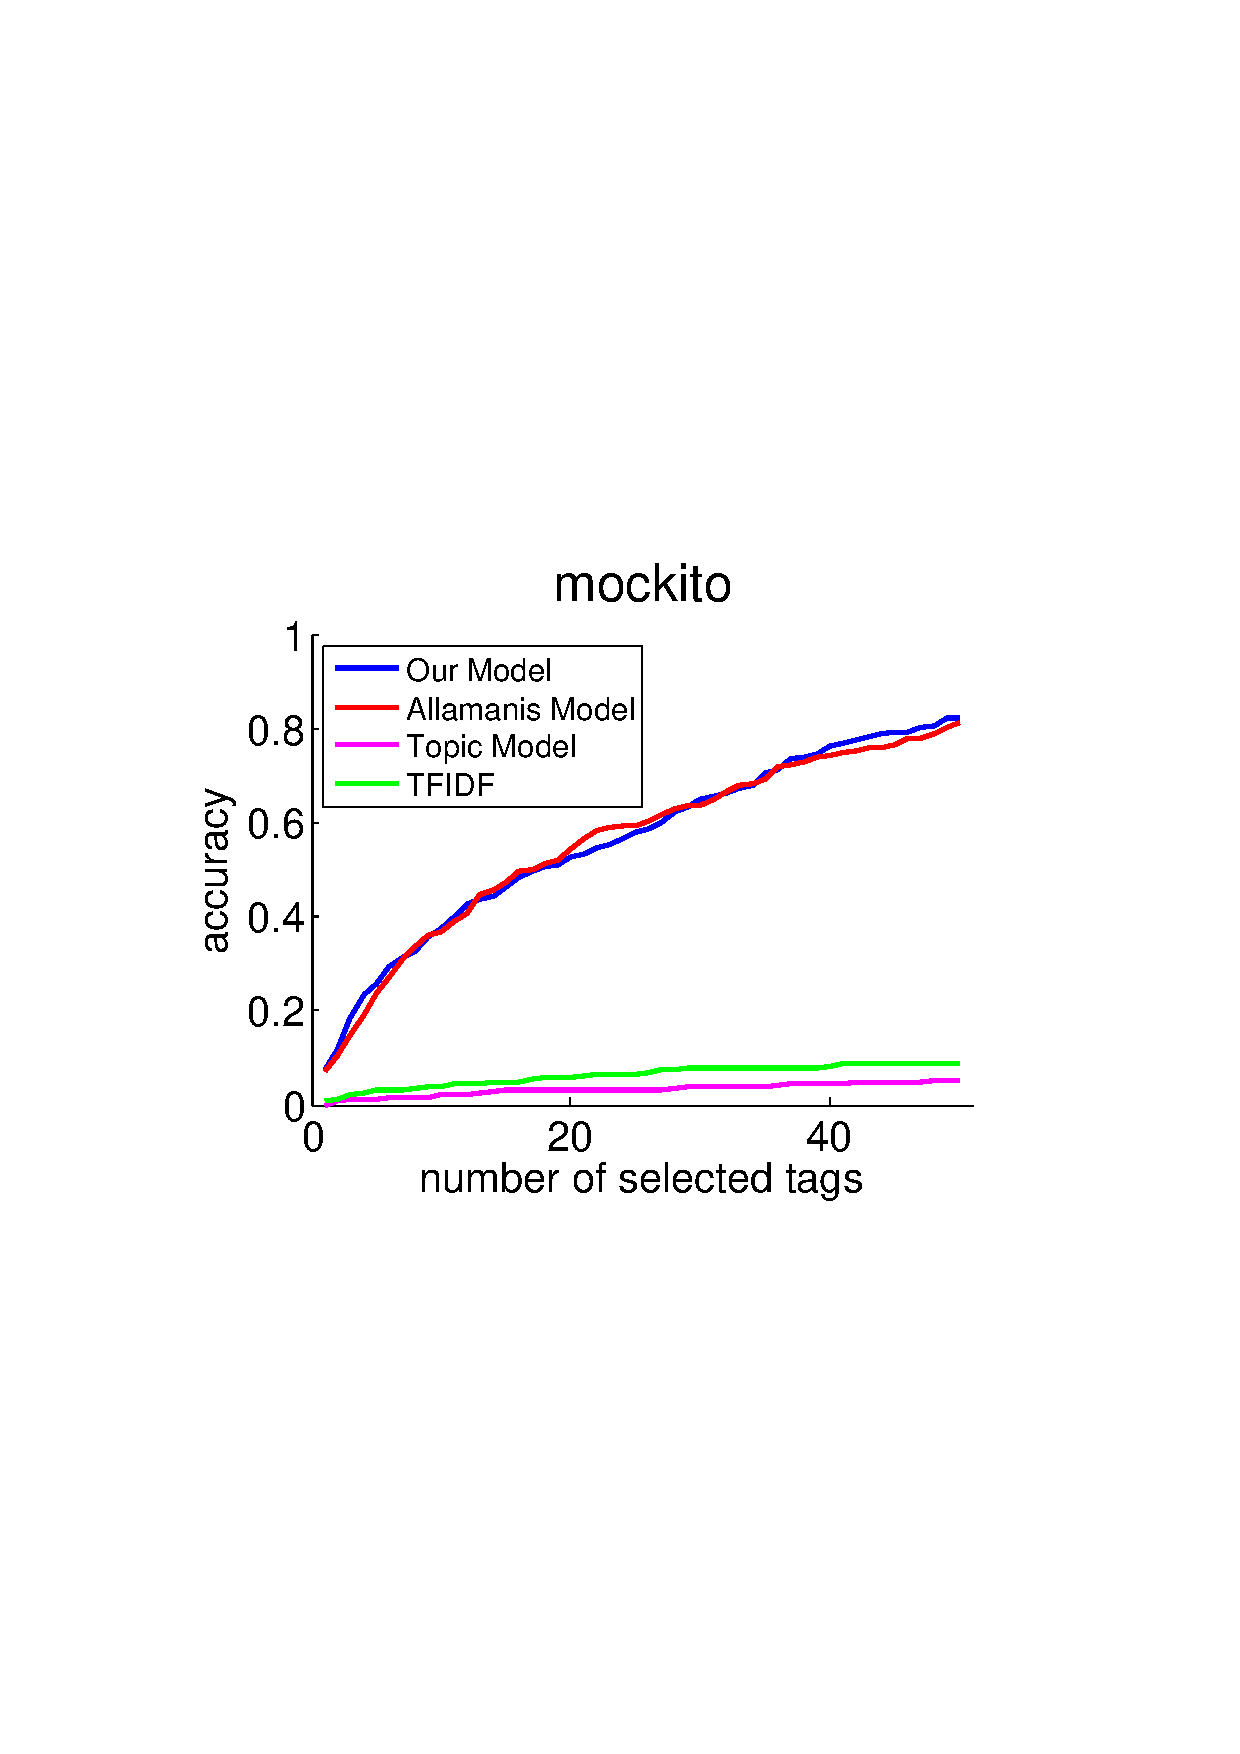
\includegraphics[width=\linewidth]{img/mockitoLine.pdf}
 \end{minipage}
 \vfill
 \begin{minipage}{0.40\linewidth}
 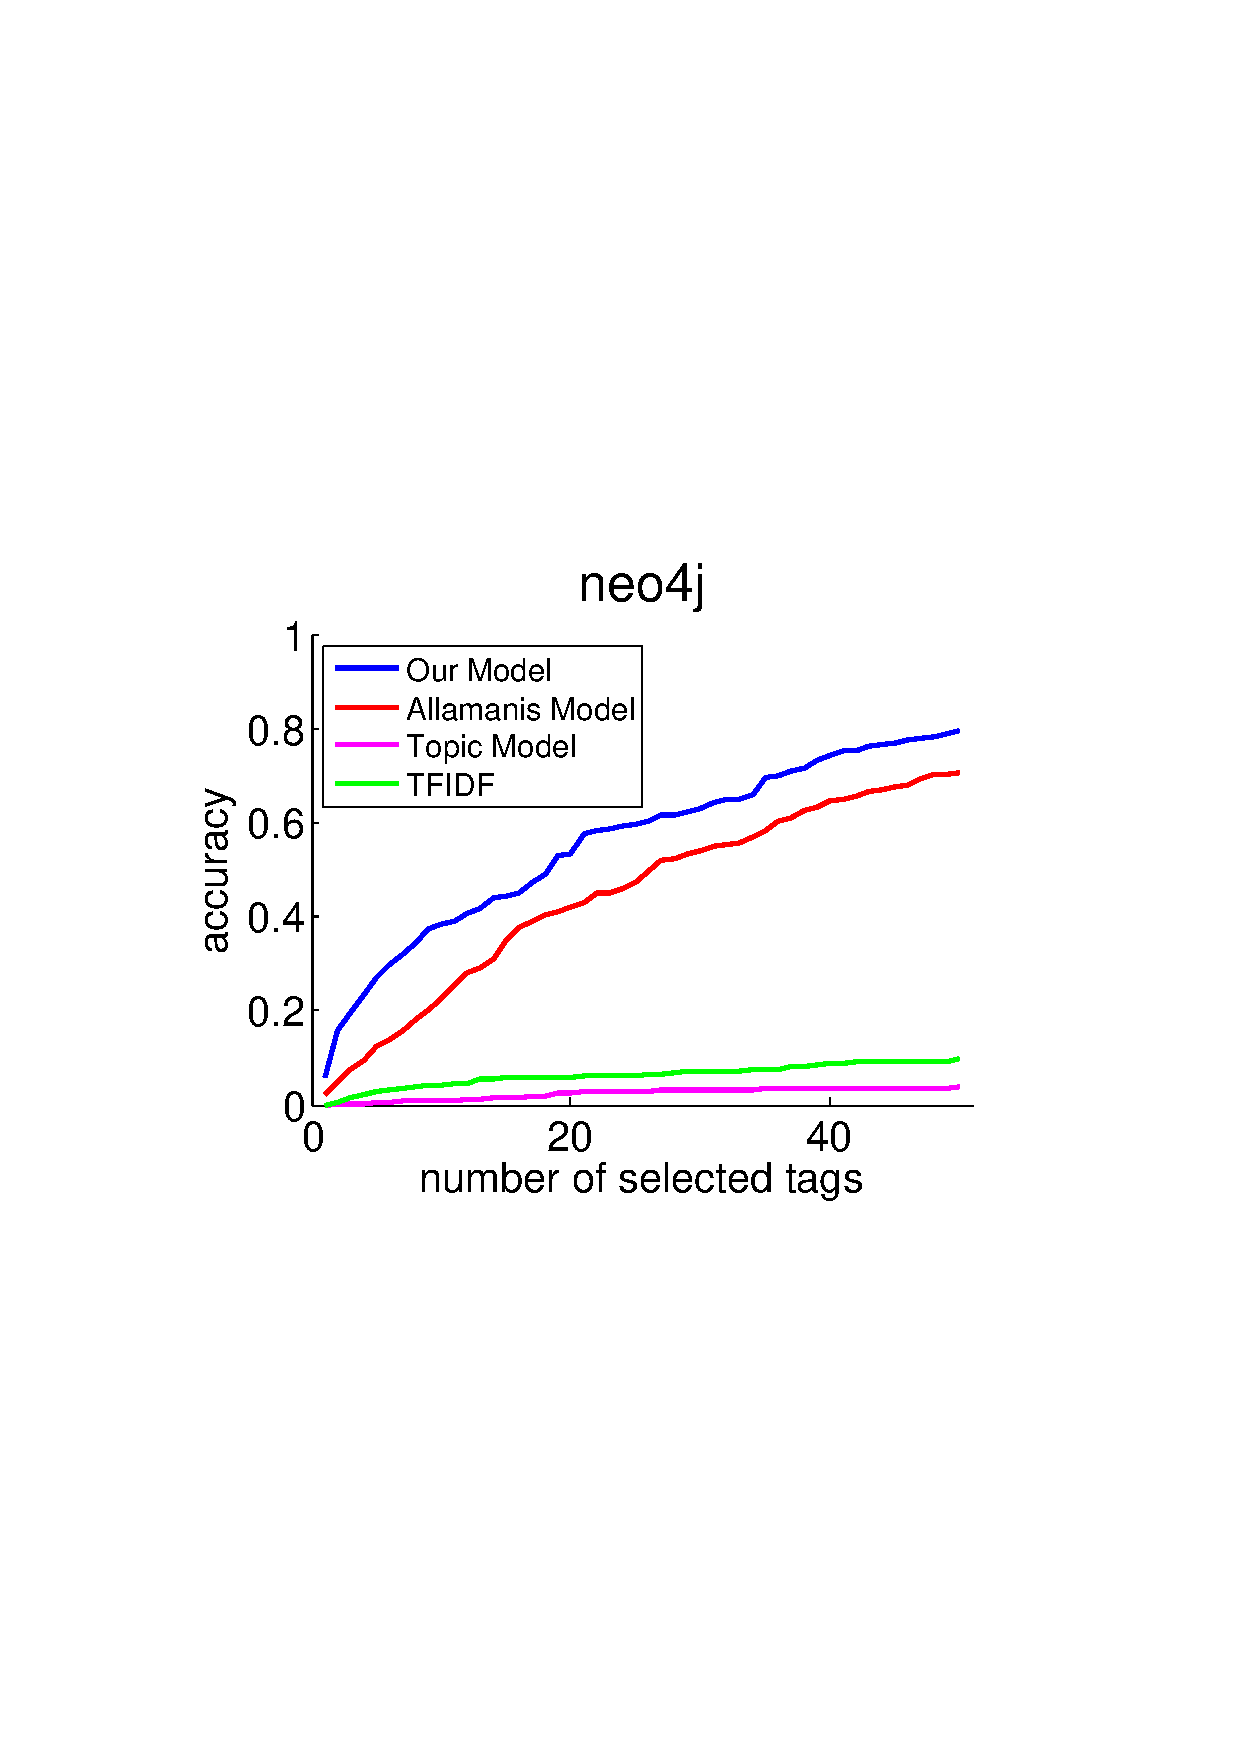
\includegraphics[width=\linewidth]{img/neo4jLine.pdf}
 \end{minipage}
 \hfill
 \begin{minipage}{0.40\linewidth}
 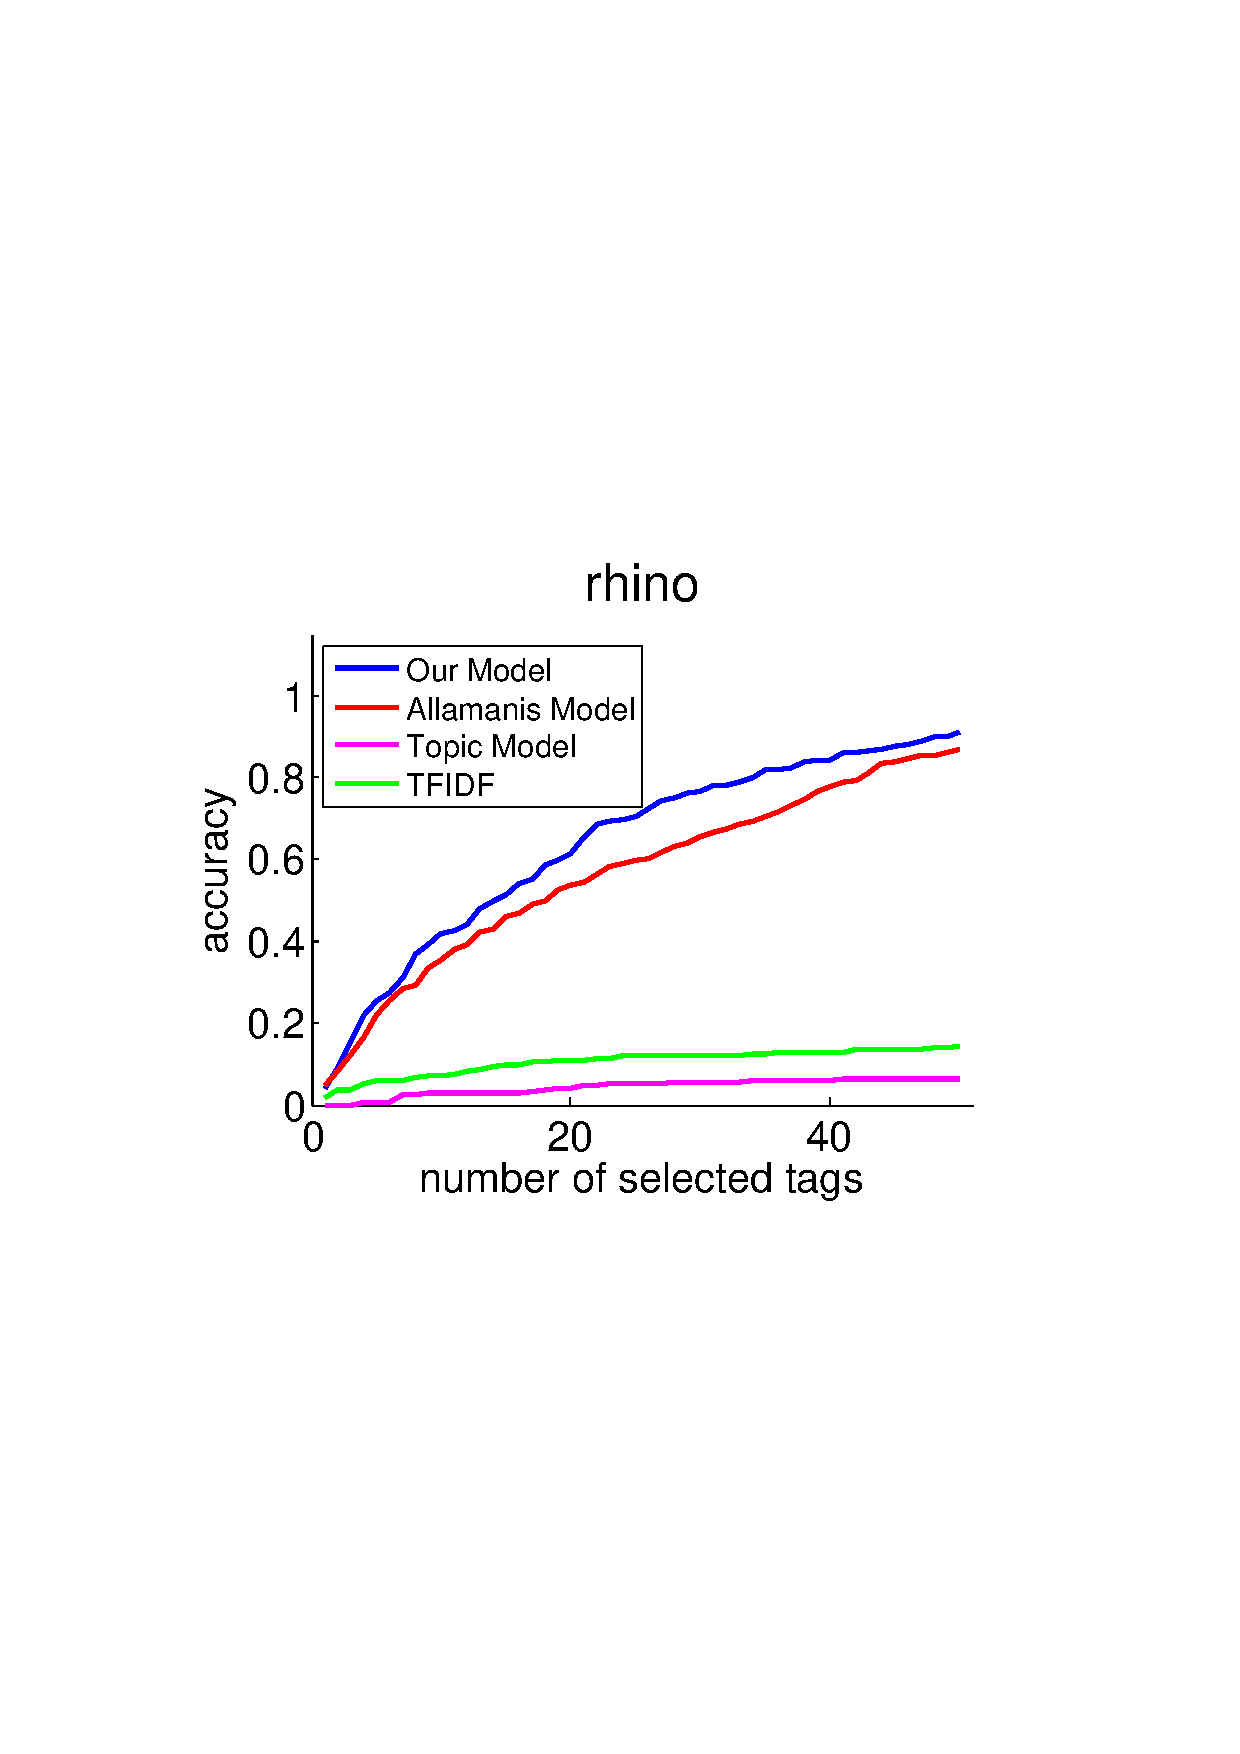
\includegraphics[width=\linewidth]{img/rhinoLine.pdf}
 \end{minipage}
 \vfill
 \begin{minipage}{0.40\linewidth}
 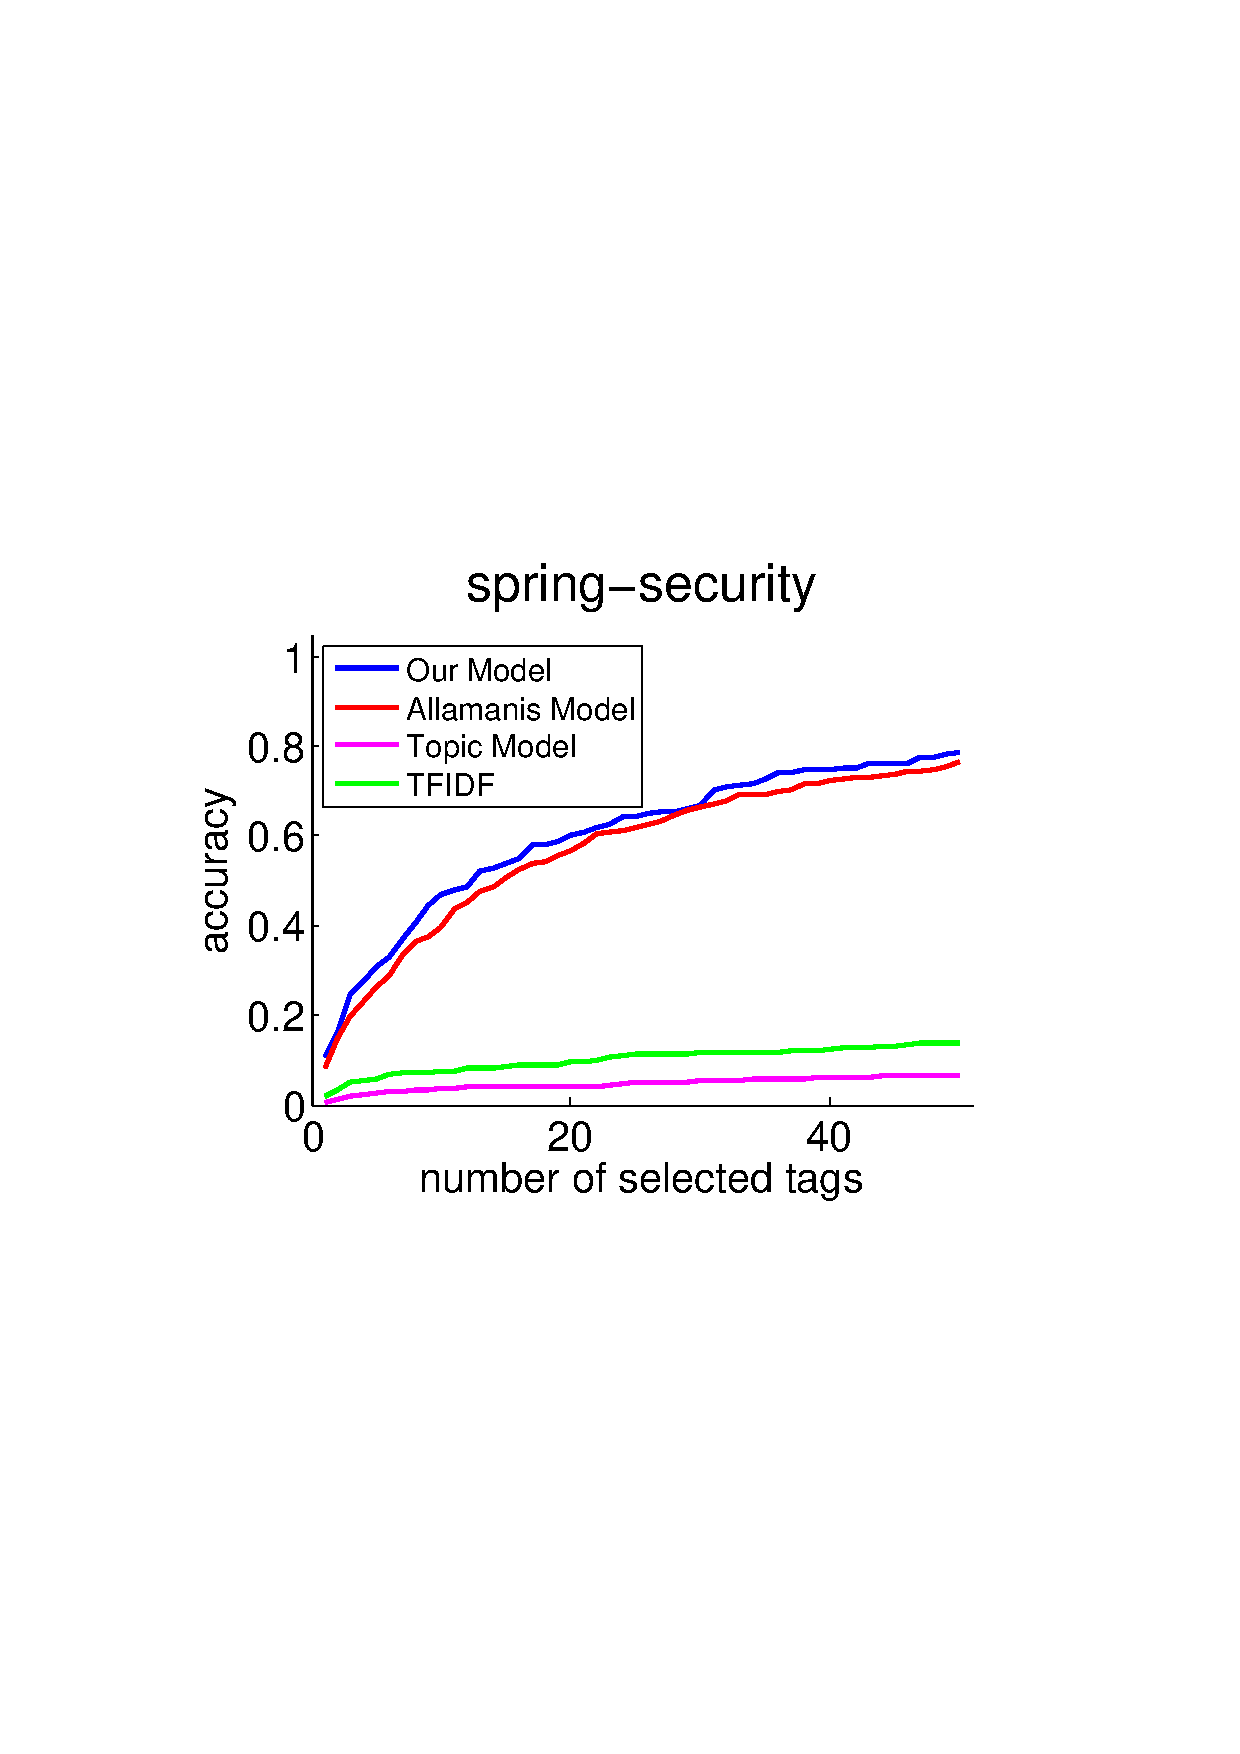
\includegraphics[width=\linewidth]{img/spring-securityLine.pdf}
 \end{minipage}
 \hfill
 \begin{minipage}{0.40\linewidth}
 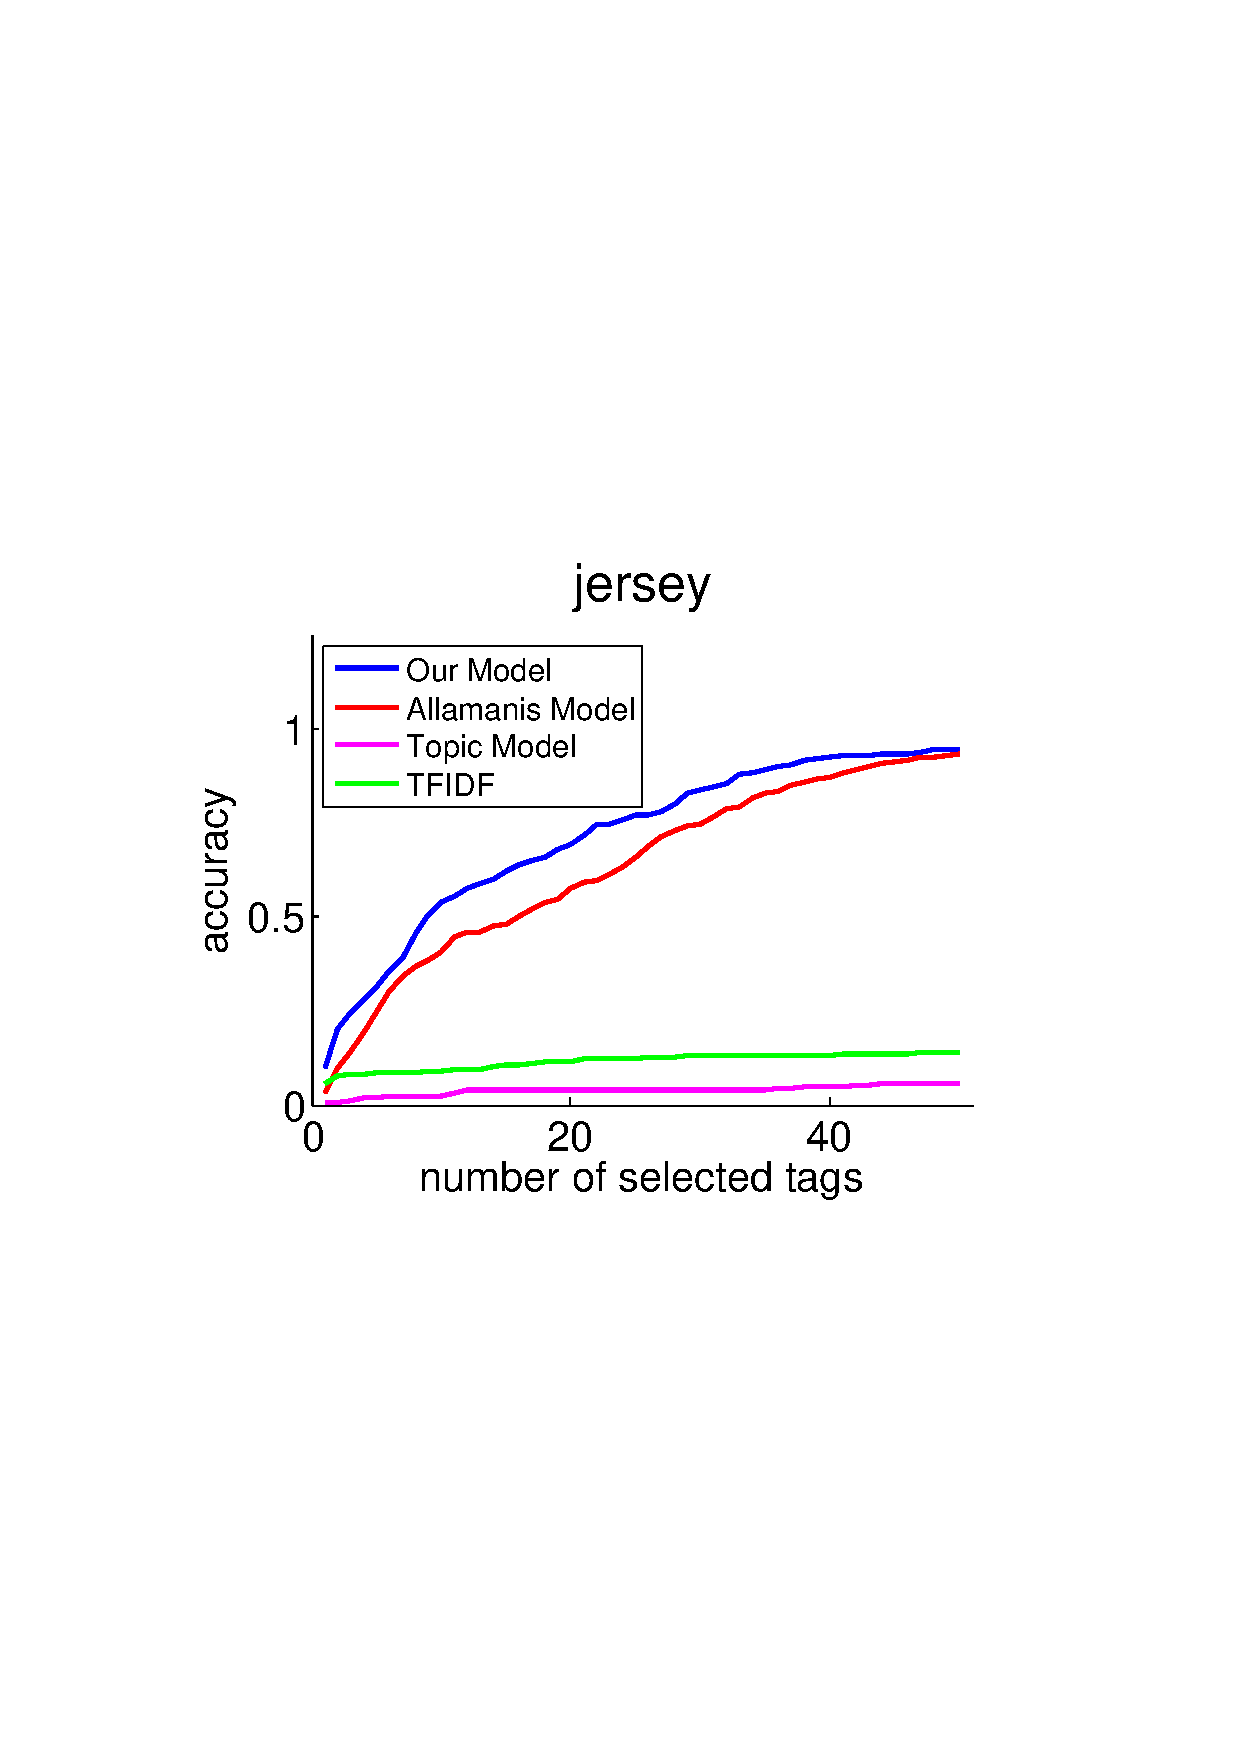
\includegraphics[width=\linewidth]{img/jerseyLine.pdf}
 \end{minipage}
 \caption{\label{figure:accuracyOfDiffTags} accuracy of different number of tags}
\end{figure}

\subsubsection{MRR}
We further compute the MRR(Mean reciprocal rank) of the ranked list of
tags of our model and Allamanis's model. For this comparison,
the tags are phrases, instead of individual words.
%When we calculate MRR, we firstly get tags that from the same function name together as a group and rank them with other groups. For example, if there are tow functions whose names are ``readBuffer'' and ``getNumber''. We can get four tags ``read'', ``buffer'', ``get'' and ``number''. And we make ``read'' and ``buffer'' in one group and ``get'' and ``number'' in one group. So our result of ranking is `` read buffer'' and ``get number''.
%the first one is read and buffer, the second one is get and number.
%By the way, because of group, number of candidates becomes 50 for every function.
Fig \ref{figure:resultMRR} shows the MRRs of 10 different source code
repositories. We can see that our model's average MRRs are better than Allamanis et al's model on all 10 repositories. %, and on some repositories our result is double of Allamanis et al's model.

\begin{figure}[ht]
 \centering
 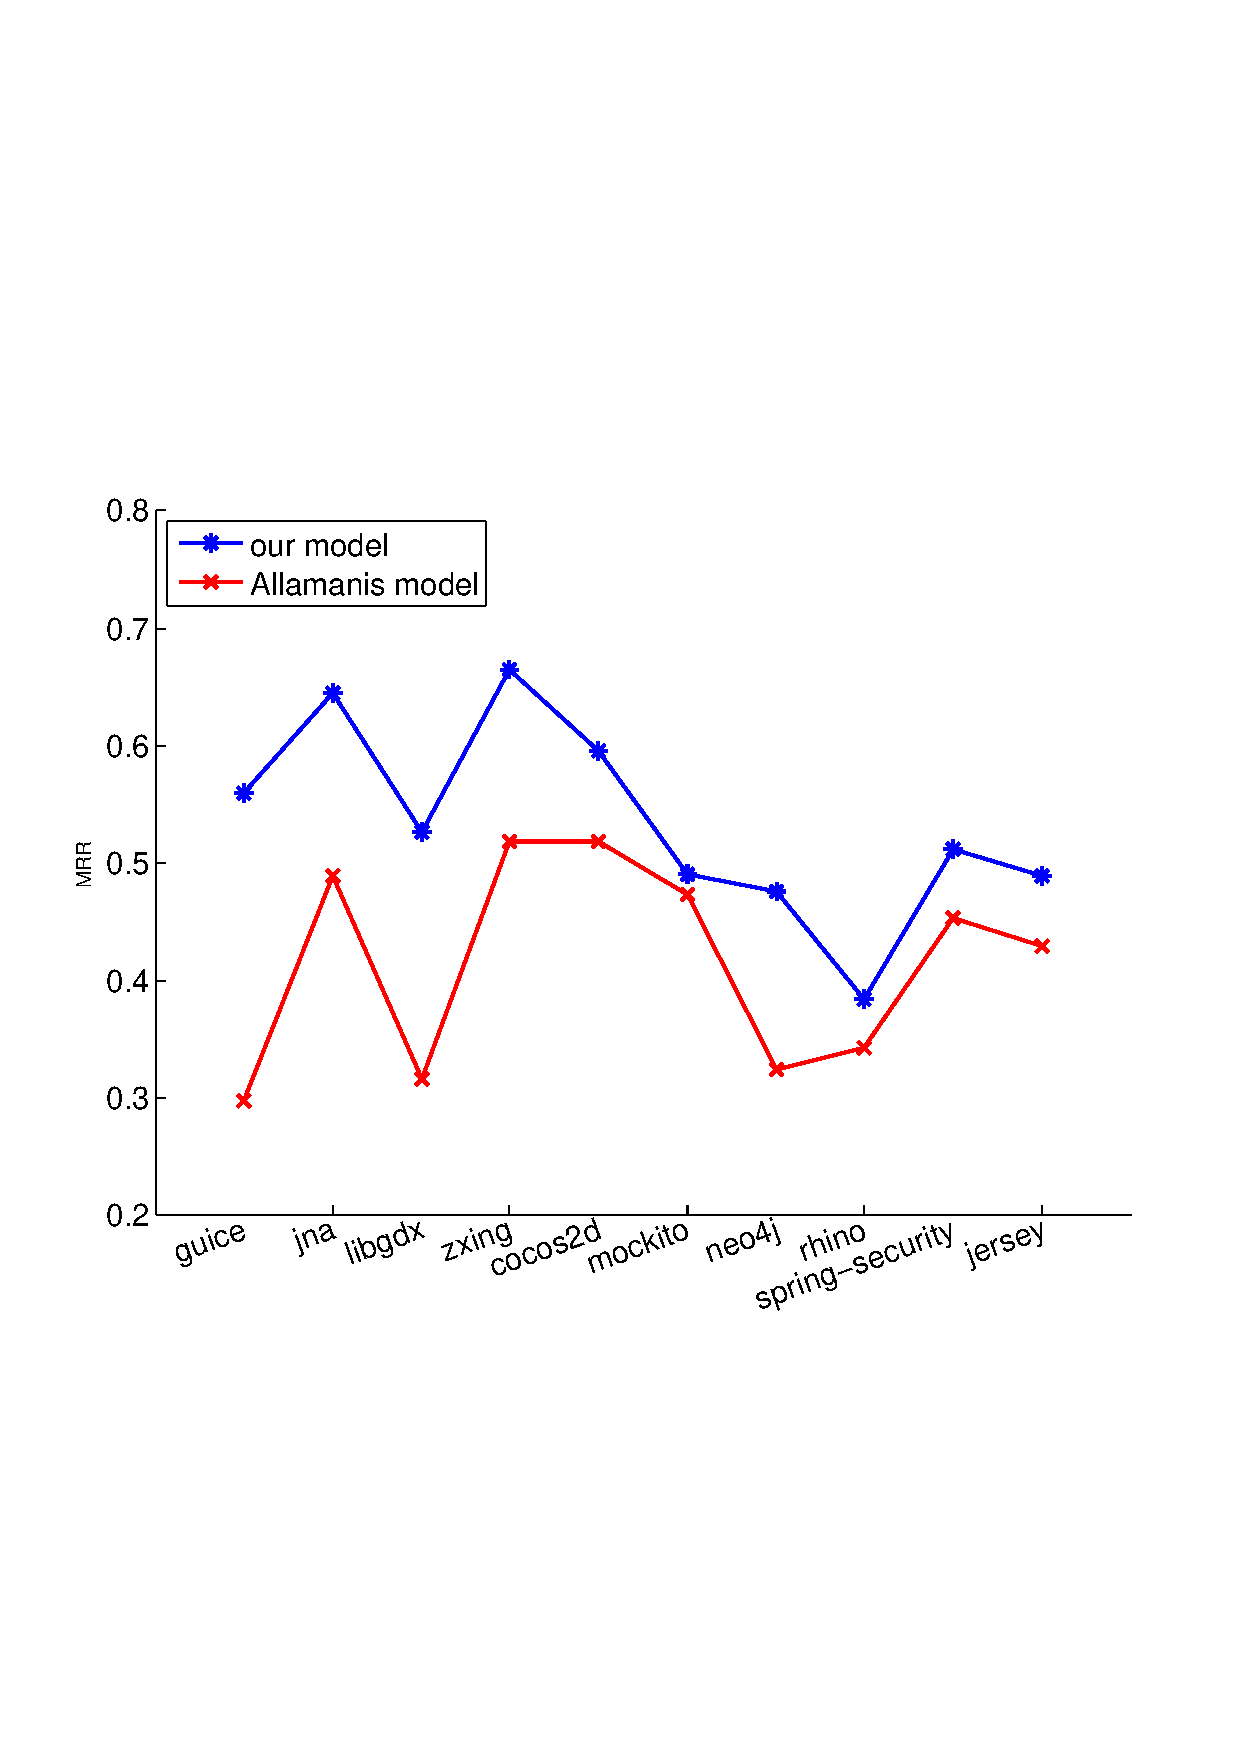
\includegraphics[width=0.8\linewidth]{img/MRR.pdf}
 \caption{\label{figure:resultMRR} MRR of Two Models}
\end{figure}

\subsubsection{With or without comments}
While comments in the source code generally provide
useful information about the source codes, some comments are just the
code that were commented out by the programmer and this kind of comments
do more harm than good.
%Wether comments is useful is based on the quality of comments. If comments contains much meaningful information of function, the result will be better with comments. On the contrary, the result will be worse if the comment is source code that were given up by programmer.
After removing such ``code'' comments from the training data,  we compare
the MRR results with or without modeling comments in
Fig \ref{figure:MRRComments}. We can see that except for repositories
neo4j and rhino, all the other results are improved after adding comments.
By observation of neo4j and rhino, we discovered that these two repositories
contain other useless comments. For example, neo4j contains many uninformative
comments that are either made up of single words like ``given'', ``when''
and ``then'' or meaningless expression such as  ``can be a file name.''
At this point, we have not developed special rules to eliminate these
useless comments
%if the quality of comments is bad and most of comments are source code that were given up by programmer, the result won't be improved or even a little worse.
%Source code repository guice's comments are an example of bad comments. Guice's comments can't help to gain the function of method. And zxing's comments is the good example of comments, these comments help model to extract much more meaningful information about the function of methods.
%Some examples about good and bad comments are shown in Table \ref{table:comments}.
%We can see that the comments from guice repository only tell us human can see some examples at which place but don't tell us any information about function of method, so this kind comment won't improve the performance of our model.
\begin{figure}[ht]
 \centering
 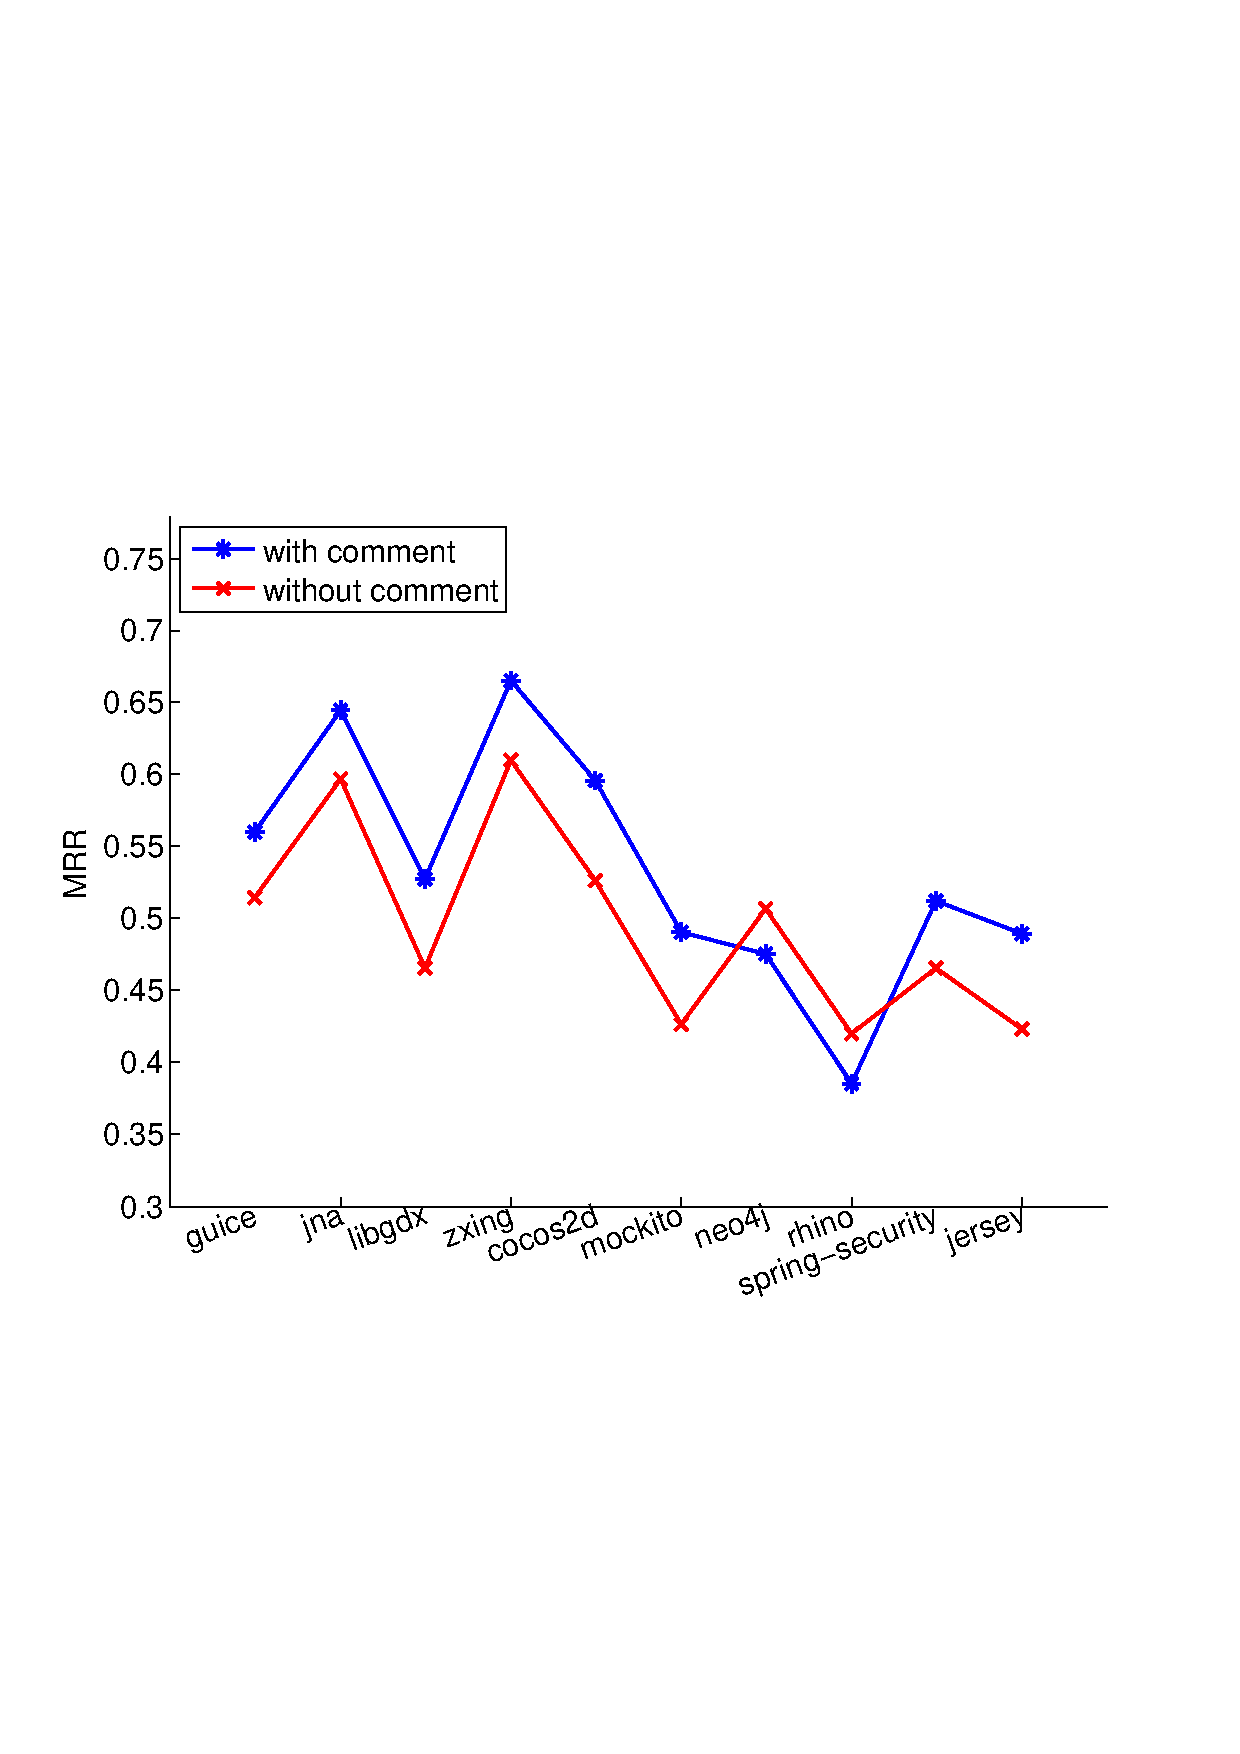
\includegraphics[width=0.8\linewidth]{img/CompareComment.pdf}
 \caption{\label{figure:MRRComments} MRR of with/without comments}
\end{figure}


\subsubsection{End-to-end Tagging Result}
We show the top 10 tags from the two competing models for
three example functions in Table \ref{table:MRRExample}.
From the first function, we can see that the true tag is at
the second position in our model and the first one is ``set.''
The tag ``set'' is related to the subject of function
``setRelativeAnchorPoint'', so to put it in the first position is reasonable.
On the other hand, the result from the Allamanis model
is much worse, the groundtruth is at the fifth position
and the first recommended tag is ``set center.''
Obviously, the word ``center'' isn't related to subject.
The second function is about picture and most of recommended tags in our model are related to it such as ``get rotation'' and ``set texture'', while the most of recommended tags in Allamanis et al's model are like ``get action'' and ``get world vector''.

%The third function in table is too long, we only put part of them and the results of two models are same, the first position.
%In the result of Allamanis et al's model for the third function, there are no true tags in the top 10 recommended tags while the true tag is at forth position in our model.


%\begin{figure}[!htp]
%\centering
%\begin{minipage}{0.49\linewidth}
% 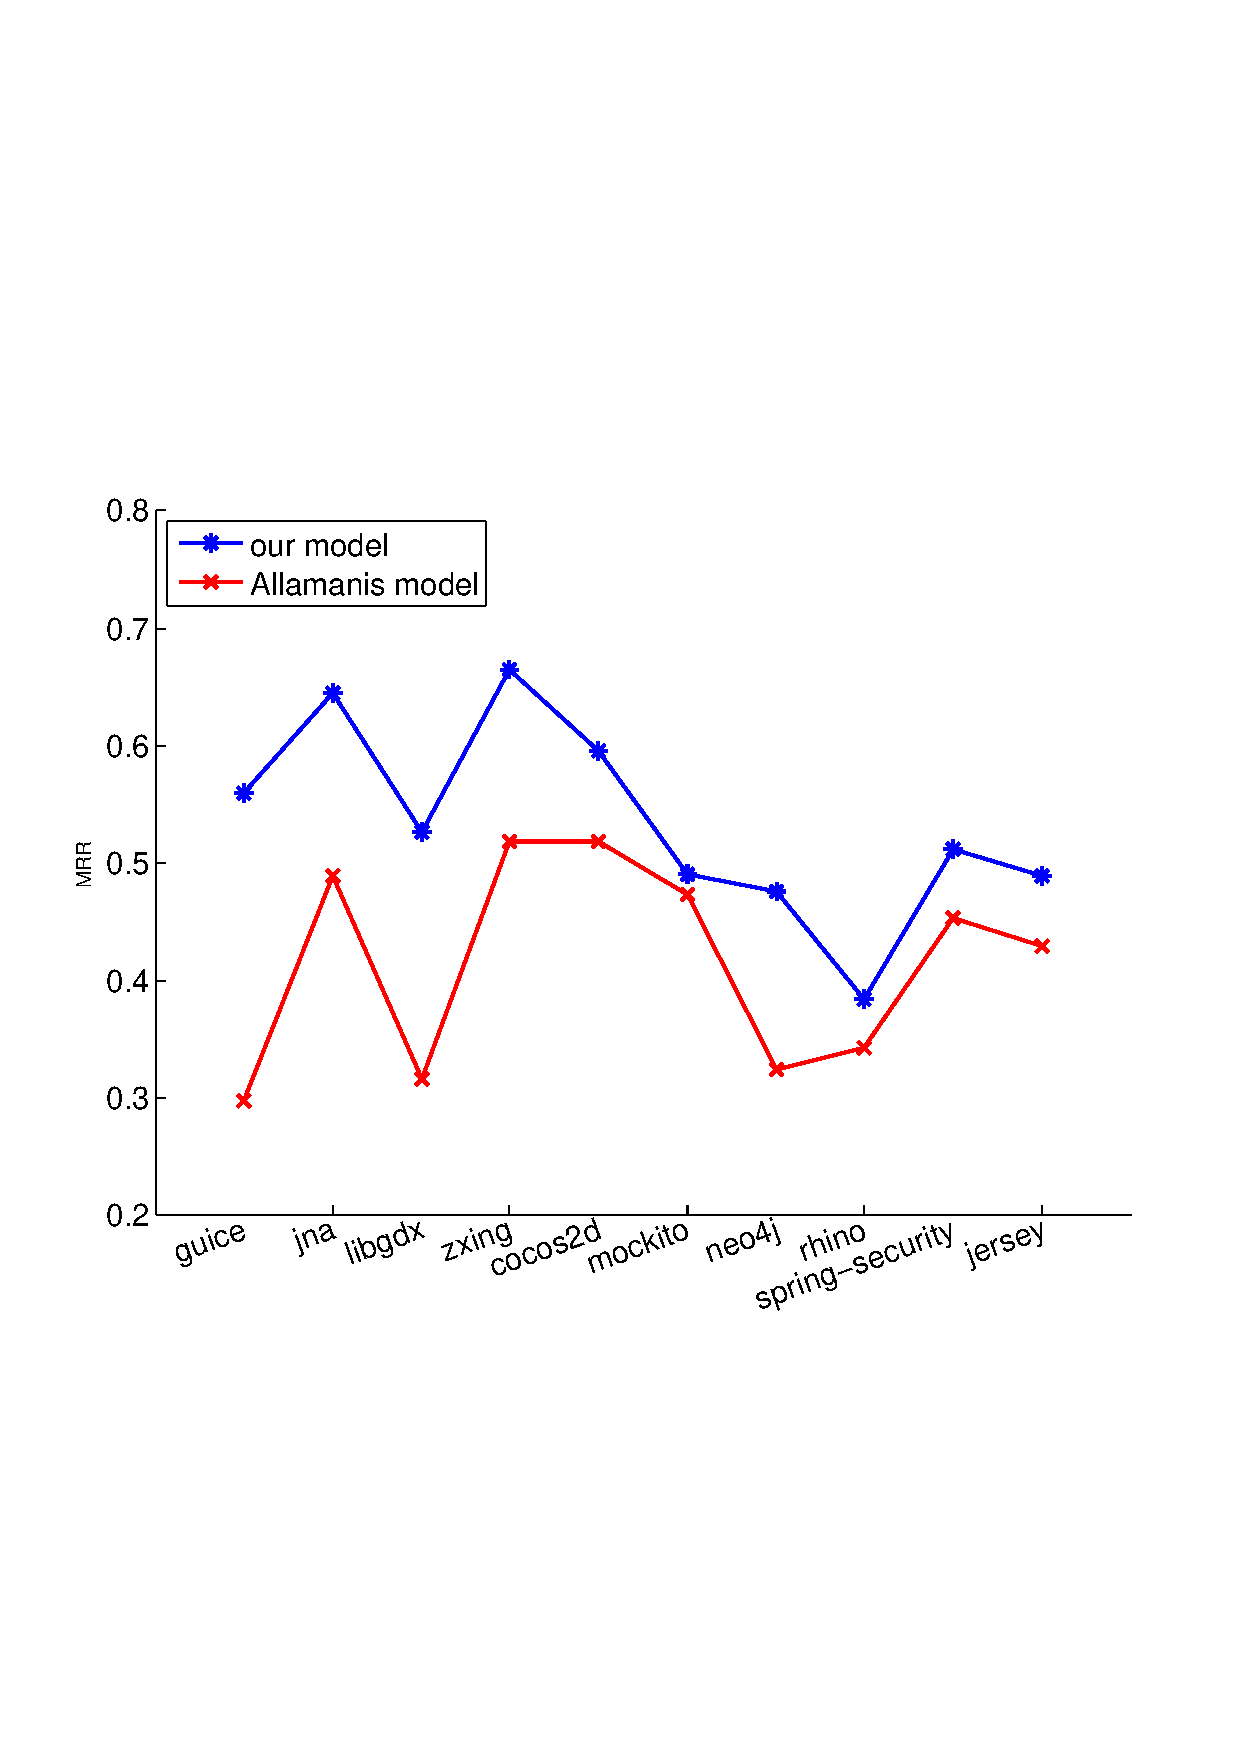
\includegraphics[width=\linewidth]{img/MRR.pdf}
% \caption{\label{figure:resultMRR} \small{result of MRR}}
% \end{minipage}
% \hfill
% \begin{minipage}{0.49\linewidth}
% 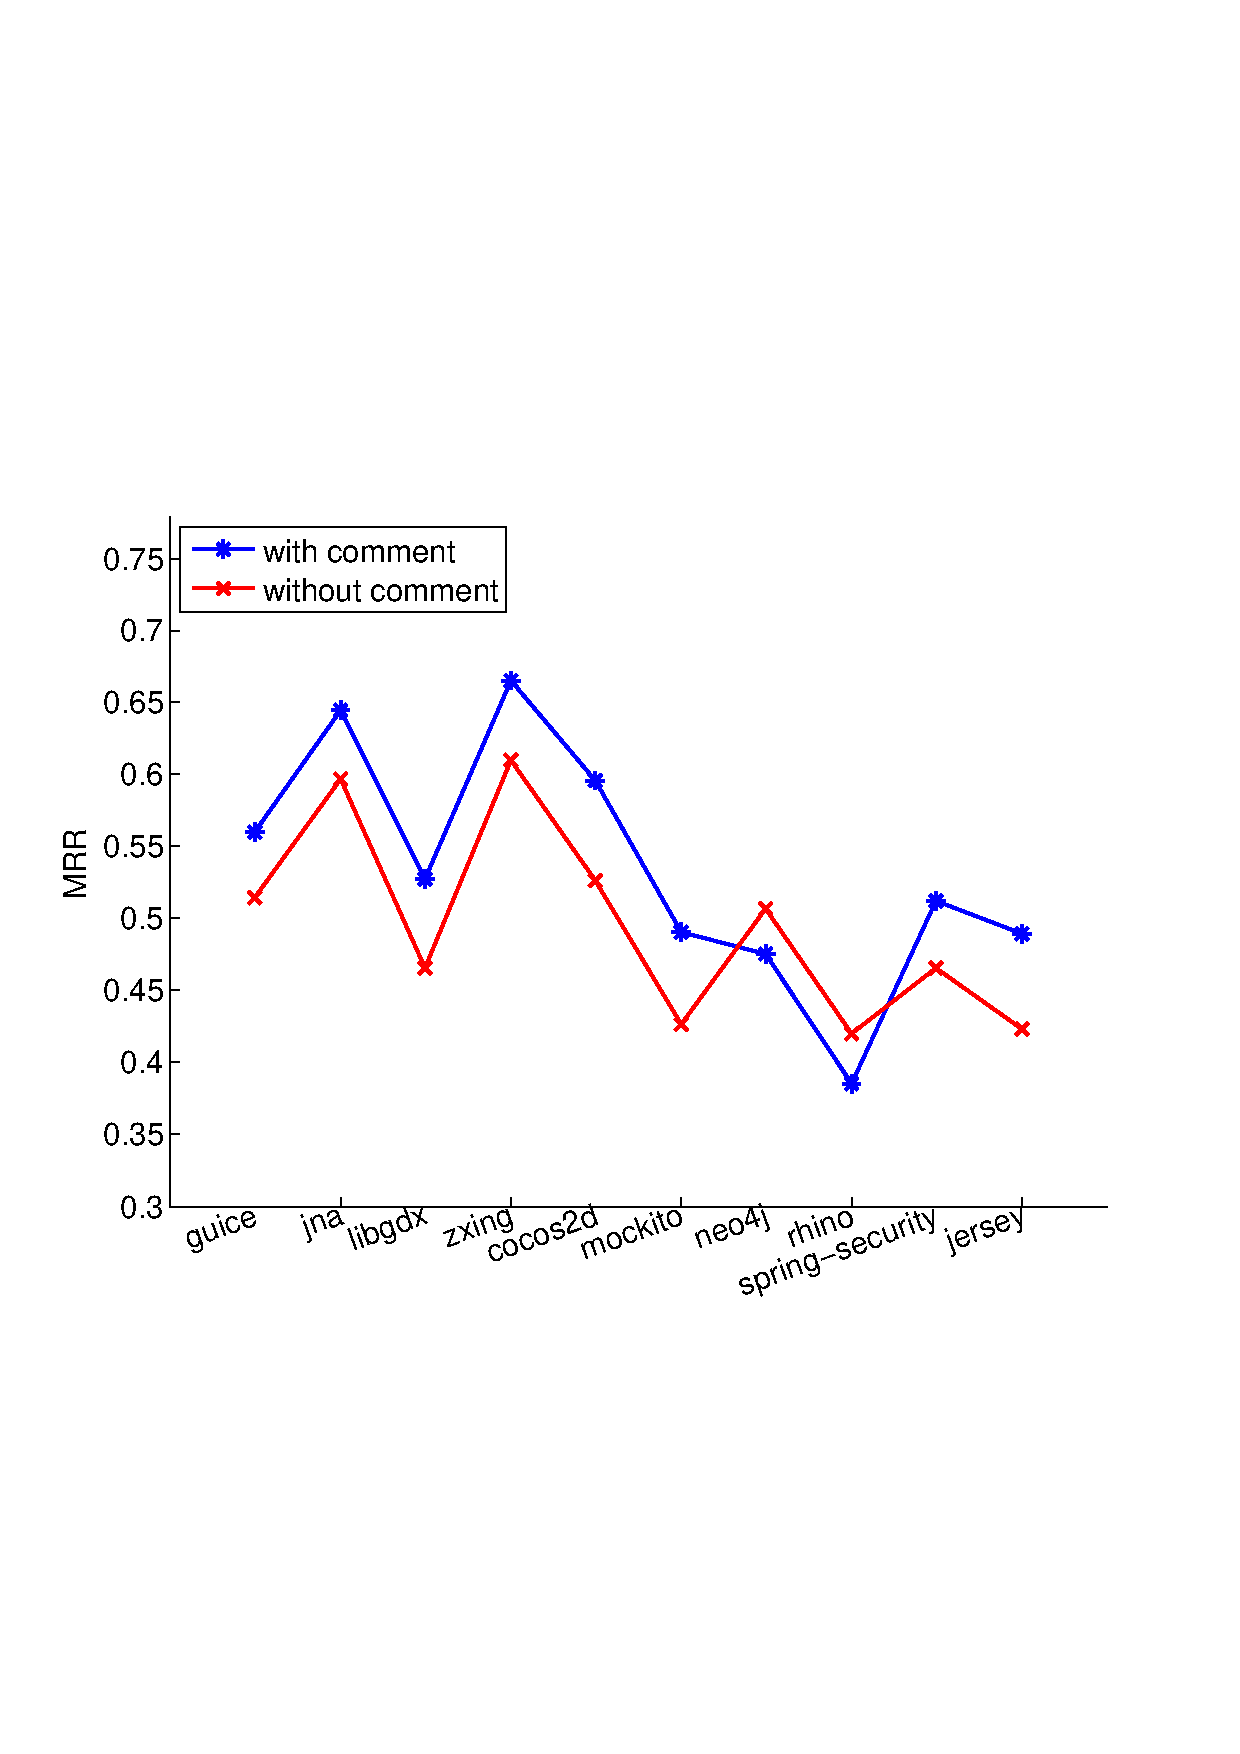
\includegraphics[width=\linewidth]{img/CompareComment.pdf}
% \caption{\label{figure:MRRComments} \small{MRR of with/without comments}}
% \end{minipage}
%\end{figure}

%\begin{table*}[!htbp]
%\centering
%\tiny{
%\caption{ \label{table:comments} Example of good and bad comments}
%\begin{center}
%\begin{tabular}{|p{10cm}|p{0.5cm}|p{5.5cm}|}
%\hline
%Example & Good or Bad & Source file\\
%\hline
%& & \\
%%\multirow{3}{*}{
%\begin{lstlisting}
%public interface OverriddenModuleBuilder {
%/**
%* See the EDSL example at {@link Modules#override(Module[]) override()}.
%*/
%Module with(Module... overrides);
%/**
%* See the EDSL example at {@link Modules#override(Module[]) override()}.
%*/
%Module with(Iterable<? extends Module> overrides);
%}
%\end{lstlisting}
%%}
% & Bad & guice/core/src/com/google/inject/util/Modules.java
% \\
%
%\hline
%%& & \\
%%\begin{lstlisting}
%%public boolean isRange(int start, int end, boolean value) {
%%if (end < start) {
%%throw new IllegalArgumentException();
%%}
%%if (end == start) {
%%return true; // empty range matches
%%}
%%end�C; // will be easier to treat this as the last actually set bit �C inclusive
%%int firstInt = start / 32;
%%int lastInt = end / 32;
%%for (int i = firstInt; i <= lastInt; i++) {
%%int firstBit = i > firstInt ? 0 : start & 0x1F;
%%int lastBit = i < lastInt ? 31 : end & 0x1F;
%%int mask;
%%if (firstBit == 0 && lastBit == 31) {
%%mask = -1;
%%} else {
%%mask = 0;
%%for (int j = firstBit; j <= lastBit; j++) {
%%mask |= 1 << j;
%%}
%%}
%%// Return false if we��re looking for 1s and the masked bits[i] isn��t all 1s (that is,
%%// equals the mask, or we��re looking for 0s and the masked portion is not all 0s
%%if ((bits[i] & mask) != (value ? mask : 0)) {
%%return false;
%%}
%%}
%%return true;
%%}
%%\end{lstlisting} & Good & zxing/core/src/main/java/com/google/zxing/common/BitArray.java
%%\\
%%
%%
%%\hline
%& & \\
%\begin{lstlisting}
%/** Reduces the size of the array to the specified size. If the array is already smaller than the specified
%size, no action is
%* taken. */
%public void truncate (int newSize) {
%cocos2d/cocos2d-android/
%if (size <= newSize) return;
%Good
%src/com/badlogic/
%for (int i = newSize; i < size; i++)
%gdx/utils/Array.java
%items[i] = null;
%size = newSize;
%}
%\end{lstlisting} & Good & cocos2d/cocos2d-android/src/com/badlogic/gdx/utils/Array.java
%\\
%\hline
%\end{tabular}
%\end{center}
%}
%\end{table*}

\begin{table}[ht]
    \centering
    \scriptsize{
    \caption{\label{table:MRRExample} Example Output Tags from Our and
Allamanis Model}
    \begin{tabular} {|p{3.6cm}|p{3.6cm}|}
    \hline
    \multicolumn{2}{|p{7.2cm}|}{ \centering Function} \\
    \hline
    \multicolumn{2}{|p{7.2cm}|}{
    Public void setRelativeAnchorPoint(Boolean newValue) \{ }\\
    \multicolumn{2}{|p{7.2cm}|}{\  \ \  \  isRelativeAnchorPoint = newValue; }\\
    \multicolumn{2}{|p{7.2cm}|}{\  \ \  \  isTransformDirty\_ = isInverseDirty+ = true;  }\\
	\multicolumn{2}{|p{7.2cm}|}{\  \ \  \ if (ccConfig.CC\_NODE\_TRANSFORM\_USING\_AFFINE\_MATRIX)\{ }\\
	\multicolumn{2}{|p{7.2cm}|}{\  \ \  \ \  \ \  \ \	isTransformGLDirty\_ = true;  }\\
	\multicolumn{2}{|p{7.2cm}|}{\  \ \  \  \}}   \\
    \multicolumn{2}{|p{7.2cm}|}{\}  }\\
    \hline
    Our model & Allamanis's model \\
    \hline
    set, \textbf{set relative anchor point}, & set center, get motor torque,\\
    %\textbf{set relative anchor point} & get motor torque \\
    get radius, get body count, & table cell at index, get next,\\
    %get body count & get next\\
    get device orientation, get next, & \textbf{set relative anchor point}, set angle, \\
	%get next & conver to ui\\
	get world center, get translation, & conver to ui, set texture, \\
	%get translation & set texture \\
    get texture rect rotated, set cqpoint & get texture, set limits \\
    %set cqpoint & set limits \\
    \hline
    \multicolumn{2}{|p{7.2cm}|}{ \centering Function} \\
    \hline
    \multicolumn{2}{|p{7.2cm}|}{public ccColor3B getColor()\{ }\\
    \multicolumn{2}{|p{7.2cm}|}{\  \ \  \ return ccColor3B.ccc3(color.r, color.g, color.b); } \\
    \multicolumn{2}{|p{7.2cm}|}{\} } \\
    \hline
    our model result & Allamanis's model \\
    \hline
    \textbf{get color}, get value, & set, \textbf{get color}, \\
    %get value & \textbf{get color}\\
    get blend func, get rotation, & get center, get action, \\
    %get rotation & get action \\
    tile, get tangent normals, & get restitution, get target, \\
    %get tangent normals & get target \\
    get tex env param, set length,& get joint list, get normals, \\
    %set length & get normals \\
    set texture, action & get world vector, get priority\\
    %action & get priority\\
    \hline
    \multicolumn{2}{|p{7.2cm}|}{ \centering Function} \\
    \hline
    \multicolumn{2}{|p{7.2cm}|}{public double getMaxDensity() \{ }\\
    \multicolumn{2}{|p{7.2cm}|}{\  \ \  \   return maxDensity; }\\
    \multicolumn{2}{|p{7.2cm}|}{ \} }\\
    \hline
    our model result & Allamanis's model \\
    \hline
    get body, get text coords, & set motor speed, set y, \\
    %get text coords & set y \\
    get blend func, \textbf{get max density}, & set tile, get next, \\
    %\textbf{get max density}& get next \\
    get position, get scale, & get aabb, get joints, \\
    %get scale& get joints \\
    set opacity, get tex env param, & set to ortho, set priority, \\
    %get tex env param & set priority \\
    get tangent normals, set to translation & get color, is motor enabled \\
    %set to translation & is motor enabled \\
    \hline
    \end{tabular}
    }
\end{table}

%\begin{table*}[ht]
%    \centering
%    \tiny{
%    \caption{\label{table:MRRExample} Example of the result to calculate MRR  }
%    \begin{tabular} {|p{10cm}|p{3cm}|p{3cm}|}
%    \hline
%    Function & our model result & Miltiadis's model\\
%    \hline
%    & & \\
%    & set & set center\\
%    & \textbf{set relative anchor point} & get motor torque \\
%    Public void setRelativeAnchorPoint(Boolean newValue) \{ &get radius & table cell at index\\
%    \  \ \  \  isRelativeAnchorPoint = newValue; & get body count & get next\\
%    \  \ \  \  isTransformDirty\_ = isInverseDirty+ = true;  & get device orientation & \textbf{set relative anchor point} \\
%	\  \ \  \ if (ccConfig.CC\_NODE\_TRANSFORM\_USING\_AFFINE\_MATRIX) \{ & get next & conver to ui\\
%	\  \ \  \ \  \ \  \ \	isTransformGLDirty\_ = true;  & get world center & set angle \\
%	\  \ \  \  \}   &  get translation & set texture \\
%    \} & get texture rect rotated & get texture \\
%    & set cqpoint & set limits \\
%    & & \\
%    \hline
%
%    & & \\
%& \textbf{get color} & set \\
%& get value & \textbf{get color}\\
%& get blend func & get center \\
%& get rotation & get action \\
%    public ccColor3B getColor()\{ & tile & get restitution \\
%    \  \ \  \ return ccColor3B.ccc3(color\_\.r, color\_\.g, color\_\.b); & get tangent normals & get target \\
%    \} & get tex env param& get joint list \\
%& set length & get normals \\
%& set texture & get world vector\\
%& action & get priority\\
%
%    & & \\
%    %\hline
%%
%%    & & \\
%%
%%    private long createProperJoint(JointDef def) \{ & \textbf{create proper joint}& \textbf{create proper joint} \\
%%  \  \ \  \  if (def.type == JointType.DistanceJoint) \{ & get next & get\\
%%  \  \ \  \ \  \ \  \  DistanceJointDef d = (DistanceJointDef) def; & get damping ratio & set position \\
%%  \  \ \  \ \  \ \  \ \  return jniCreateDistanceJoint(addr,d.bodyA.addr,d.bodyB.addr,d.collideConnected, & convert to world space & set opacity modify rgb\\
%%  \  \ \  \ \  \ \  \  \  \ \  \ d.localAnchorA.x,d.localAnchorA.y,d.localAnchorB.x,d.localAnchorB.y & get world manifold & get x \\
%%  \  \ \  \ \  \ \  \ \  \ \  \   ,d.length,d.frequencyHz,d.dampingRatio);  & get density & set color\\
%%    & to double pow & get running scene\\
%%  \  \ \  \  \} & get contact register & get percentage \\
%%
%%  \  \ \  \ \  \ \  \   \textbf{...} & get centroid & set radial accel \\
%%  \  \ \  \ \  \ \  \   \textbf{...} & is running& set blend func\\
%%  \  \ \  \ \  \ \  \    & & \\
%%
%%  \  \ \  \   if (def.type == JointType.WheelJoint) \{ & & \\
%%  \  \ \  \ \  \ \  \   WheelJointDef d = (WheelJointDef) def; & & \\
%%  \  \ \  \ \  \ \  \   return jniCreateDistanceJoint(addr,d.bodyA.addr,d.bodyB.addr,d.collideConnected, & & \\
%%  \  \ \  \ \  \ \  \   \  \ \  \ d.localAnchorA.x,d.localAnchorA.y,d.localAnchorB.x,d.localAnchorB.y & & \\
%%  \  \ \  \ \  \ \  \  \  \ \  \ ,d.localAxisA.x,d.enableMotor,d.maxMotroTorque, d.motorSpeed,    & & \\
%%  \  \ \  \ \  \ \ \  \ \  \ \ d.frequencyHz,d.dampingRatio);  & & \\
%%  \  \ \  \   \} & & \\
%%
%%  \  \ \  \   return 0; & & \\
%%    \} & & \\
%%    & & \\
%    \hline
%
%    & & \\
%    & get body & set motor speed \\
%& get text coords & set y \\
%& get blend func & set tile \\
%& \textbf{get max density}& get next \\
%    public double getMaxDensity() \{ & get position & get aabb \\
%  \  \ \  \   return maxDensity; & get scale& get joints \\
%    \} & set opacity & set to ortho \\
%& get tex env param & set priority \\
%& get tangent normals & get color \\
%& set to translation & is motor enabled \\
%
%    & & \\
%    \hline
%
%  %  & & \\
%%    & gl get integerv & set string \\
%%& add motion listener & on destroy \\
%%& \textbf{post step} & set visible \\
%%    private void postStep(float dt, int iterations) \{  & on resume & fill float buffer \\
%%  \  \ \  \   for (Steppable s:postStepList) \{ & draw string & set blend func \\
%%  \  \ \  \ \  \ \  \   s.step(dt,iterations); & set original target & \textbf{post step}\\
%%  \  \ \  \   \} & draw & set label \\
%%    \} & next callback& node \\
%%& add point & position for ortho at \\
%%& get anchor & set grid size \\
%%
%%    & & \\
%%    \hline
%    \end{tabular}
%    }
%\end{table*}

\subsection{Execution Performance}
 Table \ref{table:ExecutionPerformance} shows the execution times of
predicting tags for ten repositories. The running times of our model
is on average slightly faster than the original Allamanis model.

\begin{table}[!htbp]
    \centering
    \scriptsize{
    \caption{\label{table:ExecutionPerformance} Time of Execution(minutes)}
    \begin{tabular} {|c|c|c|c|c|}

    \hline
    \multirow{2}{*}{Repo Name} & \multicolumn{2}{c|}{Allamanis et al} & \multicolumn{2}{c|}{Our Model}\\
    \cline{2-5}
    & average & variance & average & variance \\
    \hline
    %guice & 19.3922 & 0.006548 & 18.84373 & 0.01188\\
    guice & 19.3922 & 0.0065 & \textbf{18.8437} & 0.0119\\
    \hline
    %jna & 9.8982 & 0.00307 & 10.63986 & 0.00463\\
    jna & \textbf{9.8982} & 0.0031 & 10.6399 & 0.0046\\
    \hline
    %libgdx & 30.41722 & 0.311287 & 29.1229 & 0.67438 \\
    libgdx & 30.4172 & 0.3113 & \textbf{29.1229} & 0.6744 \\
    \hline
    %zxing & 14.93435 & 0.010845 & 11.28726 & 0.05281\\
    zxing & 14.9344 & 0.0108 & \textbf{11.2873} & 0.0528\\
    \hline
    %cocos2d & 10.08613 & 0.00507 & 9.657 & 0.0181\\
    cocos2d & 10.0861 & 0.0051 & \textbf{9.6570} & 0.0181\\
    \hline
    %mockito & 15.25879 & 0.0116248 & 14.5430 & 0.0018956 \\
    mockito & 15.2588 & 0.0116 & \textbf{14.5430} & 0.0019 \\
    \hline
    %neo4j & 110.7484 & 14.03345 & 91.81392 & 5.15456 \\
    neo4j & 110.7484 & 14.0335 & \textbf{91.8139} & 5.1546 \\
    \hline
    %rhino & 19.4055 & 0.11517 & 15.3307 & 0.003828\\
    rhino & 19.4055 & 0.1152 & \textbf{15.3307} & 0.0038\\
    \hline
    %spring-security & 23.52948 & 0.006815 & 22.1473 & 0.00055897\\
    spring-security & 23.5295 & 0.0068 & \textbf{22.1473} & 0.0006\\
    \hline
    %jersey & 34.27995 & 0.783144 & 35.14936 & 0.52189\\
    jersey & \textbf{34.2800} & 0.7831 & 35.1494 & 0.5219\\
    \hline

    \end{tabular}
    }
\end{table}
